\documentclass[11pt]{article}
\usepackage[T1]{fontenc}
\usepackage{lmodern}
\usepackage[margin=1.08in]{geometry}
\usepackage{amsmath,amssymb,amsthm,mathtools}
\usepackage{microtype}
\usepackage{booktabs}
\usepackage{xcolor}
\usepackage{tikz}
\usetikzlibrary{arrows.meta,positioning}
\usepackage[hidelinks]{hyperref}
\usepackage{bookmark}
\usepackage{enumitem}
\setlist{itemsep=3pt,topsep=5pt}
\newtheorem{theorem}{Theorem}[section]
\newtheorem{lemma}[theorem]{Lemma}
\newtheorem{proposition}[theorem]{Proposition}
\newtheorem{corollary}[theorem]{Corollary}
\theoremstyle{definition}
\newtheorem{definition}[theorem]{Definition}
\theoremstyle{remark}
\newtheorem{remark}[theorem]{Remark}
\newcommand{\Z}{\mathbb Z}
\newcommand{\R}{\mathbb R}
\newcommand{\E}{\mathbb E}
\newcommand{\N}{\mathbb N}
\newcommand{\Prb}{\mathbb P}
\newcommand{\calH}{\mathcal H}
\newcommand{\calL}{\mathcal L}
\newcommand{\av}{\mathop{\mathrm{av}}}
\DeclareMathOperator{\TV}{TV}
\DeclareMathOperator{\supp}{supp}
\DeclareMathOperator{\diam}{diam}
\DeclareMathOperator{\dist}{dist}
\numberwithin{equation}{section}
\hypersetup{pdftitle={Bounded-Step Walks on Gaussian Primes},pdfauthor={OpenAI}}
\title{Bounded-Step Walks on Gaussian Primes}
\author{OpenAI}
\date{September 26, 2026}

\begin{document}
\maketitle
\begin{abstract}
We prove the Gaussian moat conjecture: no infinite walk through distinct
Gaussian primes can have bounded steps. More strongly, for each fixed finite
step bound, the connected components of the Gaussian-prime graph have
uniformly bounded size. This bound applies to every starting prime, including
primes on the coordinate axes, and is nonexplicit. The proof constructs a
finite periodic sieve obstruction using geometric sampling and
information-theoretic estimates.
\end{abstract}

\section{The Gaussian moat problem}\label{sec:introduction}\label{sec:intro}
A Gaussian prime is an irreducible element of $\Z[i]$.
We identify $a+bi$ with $(a,b)\in\Z^2$, write $N(a+bi)=a^2+b^2$,
and use the Euclidean norm $|z|=\sqrt{N(z)}$.
For a finite real $D$, let $G_D$ have all Gaussian primes as vertices,
with an edge between distinct $z,w$ if $|z-w|\le D$.
The Gaussian moat problem asks whether some $G_D$ contains an infinite
path with no repeated vertex. Large gaps along a line do not settle the
question in the plane, since a path may go around them.

\begin{theorem}[Uniform component bound]\label{thm:main}\label{cor:uniform}
For every finite real $D$ there is a finite $B_D$ such that every
connected component of $G_D$ has at most $B_D$ vertices.
The bound is independent of the starting prime and includes primes on
the coordinate axes. Consequently every sequence of distinct Gaussian
primes whose successive distances are at most $D$ has at most $B_D$ terms.
\end{theorem}

This proves the uniform form of the Gaussian moat conjecture and answers
the infinite-walk question negatively. The bound $B_D$ is nonexplicit:
the proof chooses
sufficiently large scales after fixing $D$. For $D<1$, distinct lattice
points cannot be adjacent, so $B_D=1$ suffices.

Gethner and Stark trace the question to Basil Gordon at the 1962
International Congress of Mathematicians in Stockholm
\cite[p.~289]{GethnerStark}. Erd\H{o}s later credited Gordon and Motzkin,
recalling that Motzkin had told him the problem at the Pasadena number
theory meeting in November 1963 \cite[p.~69]{Erdos1977}.

The early work separates two obstacles. Large prime-free disks obstruct
motion locally, but a planar walk may go around them. Gethner, Wagon,
and Wick constructed such disks with centers on any line containing two
Gaussian integers, and constructed arbitrarily isolated real Gaussian
primes; they credit Vardi with an independent proof of the latter result
\cite[Theorems 4.1 and 4.4]{GethnerWagonWick}.
Computations instead surround a particular starting region:
Tsuchimura obtained a finite bound on the distance reachable with steps
of length at most $6$ from the origin, adjoined as an initial vertex
\cite{Tsuchimura}. This is a result about the component of that vertex.

The closer predecessor of the present argument is finite periodic
sieving. Gethner and Stark formulated a bound on the length of a
distinct-prime walk that is uniform over its starting point, established
periodic obstructions for step bounds $\sqrt2$ and $2$, and proposed
sieving by small Gaussian primes for larger bounds
\cite[pp.~290--292]{GethnerStark}. Vardi studied the associated periodic
coprimality graphs and the passage from the absence of an infinite walk
to a uniform bound on component sizes
\cite[Section 6, Proposition 6.2]{Vardi}.
Our finite-sieve theorem supplies congruence restrictions for each fixed
step bound; the periodic reduction below then converts those restrictions
into the bound on all Gaussian-prime components.


\subsection{A finite obstruction and the route to its proof}
For a rational prime $p\equiv1\pmod4$, choose conjugate Gaussian prime
factors $\pi_p,\overline{\pi_p}$, each of norm $p$.
For a finite set $\mathcal P$ of such rational primes, put
\[
\mathcal A(\mathcal P)=\{z\in\Z[i]:
 z\not\equiv0\pmod{\pi_p},\quad
 z\not\equiv0\pmod{\overline{\pi_p}}\quad(p\in\mathcal P)\}.
\]
Changing the chosen associates does not change this set. It is periodic
under translations by $Q\Z^2$, where $Q=\prod_{p\in\mathcal P}p$.

\begin{theorem}[Finite sieve obstruction]\label{thm:sieve}
For every $D\ge1$ there is a finite set $\mathcal P_D$ of rational
primes congruent to $1$ modulo $4$ such that $\mathcal A(\mathcal P_D)$
contains no infinite sequence of distinct points with successive distances
at most $D$. The set $\mathcal P_D$ depends only on $D$.
\end{theorem}

Section~\ref{sec:consequences} first proves that this finite obstruction
implies Theorem~\ref{thm:main}. The remaining sections construct it.
We fix an arbitrary deterministic infinite self-avoiding lattice walk
with steps at most $D$. Randomness enters only through sampled times
and auxiliary choices of one Gaussian factor over each split prime.
The aim is to show that such a walk cannot avoid all the selected zero
classes.

The geometric sampling operation in Section~\ref{sec:geometry} chooses
a difference uniformly from the distinct differences of a long walk
segment and then chooses one of its endpoints. There are many distinct
differences, and a random collection of signed prime factors usually
separates them. These facts force the sampled endpoint to carry more
joint entropy in its residues than the earlier position did. The proof
uses a torus-degree argument for the differences, followed by determinant
divisibility and concentration for the factor choices. Disjoint
neighborhoods in the Boolean cube avoid a separate count of all lattice
directions.

The next task is coverage: for most factors of norm $p$, the terminal
residue must have probability at least $\tau/p$ outside fewer than
$p^{1-\beta}$ exceptional residues. Joint entropy alone, at the accuracy
available early in the construction, does not give this conclusion.
Section~\ref{sec:transfer} supplies the additional argument before the
large schedule of parameters is introduced. Repeated continuations from
an exact later checkpoint give one displacement vector shared by every
residue coordinate. If coverage failed, this vector would put the true
residue on a short list with appreciable probability. Its entropy cost
is too small to create that deficit in many coordinates at once.

Section~\ref{sec:schedule} arranges the geometric operations in a common
schedule with decreasing scales. It first establishes the entropy and
displacement estimates, then applies the coverage transfer backward
through the checkpoints. Every prime batch uses the same terminal time
law, denoted by $t_*$. An independent uniform offset makes this law
nearly invariant under the time shifts needed later.

Finally, assume that the walk avoids the chosen zero classes.
Section~\ref{sec:information} uses short increment words---finite lists
of consecutive increments---to test candidate starting residues.
Coverage and self-avoidance make these tests informative. Each prime
batch near $T$ incurs conditional information at least $c/\log T$ per
increment, where $c>0$ depends only on $D$. Section~\ref{sec:budget}
adds these costs using nested residue vectors and dyadic word lengths
at the common time law. Block subadditivity bounds their sum by the
entropy available in one bounded increment, whereas the selected batches
make the lower bounds diverge. This proves the finite sieve theorem.
The use of approximate translation invariance and block subadditivity
to bound accumulated information is methodologically related to Tao's
entropy-decrement argument~\cite[Section 3]{TaoEntropyDecrement}.
Here the signed residue batches, coverage transfer, and costs forced by
zero avoidance are established in full within this paper.

\section{Periodicity and the uniform bound}\label{sec:consequences}
The finite sieve theorem will be proved independently of the component
bound. The following conditional reduction explains why that theorem
suffices, and records the contribution of the finitely many Gaussian
primes removed by the sieve. The periodicity principle also appears in
Vardi~\cite[Section 6, Proposition 6.2]{Vardi}.

\begin{proposition}[From a periodic obstruction to a uniform bound]
\label{prop:periodic}
Fix $D\ge1$ and a finite set $\mathcal P$ of rational primes congruent
to $1$ modulo $4$. Suppose that $\mathcal A(\mathcal P)$ contains no
infinite self-avoiding walk with steps at most $D$. Put
\[
 Q=\prod_{p\in\mathcal P}p,\qquad
 K_D=\#\{v\in\Z[i]:|v|\le D\},
\]
and let $E$ be the set of associates of the selected Gaussian factors.
For every component $C$ of $G_D$,
\[
 \#C\le\max\{Q^2,\ |E|+(K_D-1)|E|Q^2\}.
\]
\end{proposition}
\begin{proof}
The graph on $\mathcal A(\mathcal P)$ with this step bound is locally
finite and invariant under translations by $Q\Z^2$. An infinite
component would contain an infinite simple path: the tree of finite
simple paths from one vertex is finitely branching, has vertices at
arbitrarily large depths, and one can successively choose a child with
arbitrarily deep descendants. Hence every component is finite.

Suppose that two distinct points $x,y$ of a component differ by
$v\in Q\Z^2$. Translation by $v$ sends that component to a component
containing $y$, so sends it to itself. A finite nonempty subset of
$\Z^2$ cannot be invariant under a nonzero translation. Each component
therefore injects into $(\Z/Q\Z)^2$ and has size at most $Q^2$.

A Gaussian prime divisible by a selected factor is an associate of that
factor. Thus, after deleting $E$, the Gaussian-prime graph is a subgraph
of the avoiding graph. A component meeting $E$ can meet at most
$(K_D-1)|E|$ components of the graph with $E$ removed: each such
component has an edge to $E$, whose total degree is at most that number.
Adding back $E$ gives the claimed bound.
\end{proof}


Applying Proposition~\ref{prop:periodic} to the set supplied by
Theorem~\ref{thm:sieve} proves Theorem~\ref{thm:main} for $D\ge1$;
the case $D<1$ was settled in the introduction. For the weaker
infinite-walk conclusion, one can simply delete an initial segment
containing the finitely many exceptional Gaussian primes: the remaining
tail would lie in $\mathcal A(\mathcal P_D)$.

Periodicity is what makes the bound uniform in the starting point.
Absence of an infinite path in a general locally finite graph does not
bound the sizes of its finite components. We now turn to the arithmetic,
entropy, and geometry needed to produce the finite obstruction.

\section{Arithmetic, walks, and entropy}\label{sec:preliminaries}

We record the conventions needed to sample a fixed walk and to compare
the resulting residue distributions. All logarithms are natural.
The notation \(A\ll_D B\) means \(A\le c_D B\) with a constant depending
only on \(D\); \(A\asymp_D B\) means both inequalities.
Constants without a subscript are absolute. Asymptotic statements about
a collection of walks or starting times will always be uniform over
that collection.

\subsection{Split primes}

The ring \(\Z[i]\) is Euclidean and hence has unique factorization.
For each rational prime \(p\equiv1\pmod4\), its two conjugate Gaussian
prime factors are nonassociate, have norm \(p\), and have residue fields
of size \(p\); see~\cite[Corollary 7.9 and Theorems 7.14, 9.7, 9.9]{Conrad}.
We refer to the choice of one of these two factors as a \emph{sign}.
Signs of distinct rational primes will be independent and fair.

We use the following consequences repeatedly. If \(\pi\mid v\) and
\(\overline\pi\mid v\), then \(p\mid v\), meaning that \(p\) divides both
integer coordinates of \(v\). If \(a\in\Z\), then
\(\pi\mid a\) if and only if \(p\mid a\).
Every nonzero multiple of \(\pi\) has length at least \(\sqrt p\).
Finally, multiplication by a Gaussian integer \(\alpha\) acts on
\(\Z^2\) by an integer matrix of determinant \(N(\alpha)\). Thus if
\(\alpha\mid v,w\), then
\[
\det(v,w)\in N(\alpha)\Z.
\]

For \(T>1\), let
\[
\mathcal B_T=\{p\text{ rational prime}:T\le p\le2T,\ p\equiv1\pmod4\},
\qquad k_T=|\mathcal B_T|,
\qquad L_T^*=\frac1{k_T}\sum_{p\in\mathcal B_T}\log p.
\]
All uses have \(T\) sufficiently large that \(k_T>0\).
For one fixed batch we abbreviate \(k_T,L_T^*\) by \(k,L_*\).
The prime number theorem in arithmetic progressions for the fixed
modulus \(4\) gives~\cite[Equations (1.1)--(1.2), p.~66]{Selberg}
\begin{equation}\label{eq:prime-count}
k_T=(1/2+o(1))\frac{T}{\log T},
\qquad \log T\le L_T^*\le\log(2T).
\end{equation}
Indeed Selberg's weighted asymptotic
\(\sum_{p\le x,\ p\equiv1(4)}\log p\sim x/2\), subtracted at \(T\)
and \(2T\), gives a sum over \(T<p\le2T\). Adding the possible
endpoint term at \(p=T\) changes it by at most \(\log T\). The weighted
sum over \(\mathcal B_T\) therefore equals \((1/2+o(1))T\) and lies
between \(k_T\log T\) and \(k_T\log(2T)\), whose ratio tends to \(1\).
Only fixed-modulus, fixed-ratio intervals are involved. In particular,
all constants implicit in \eqref{eq:prime-count} hold for every
sufficiently large \(T\).

\subsection{Entropy conventions}

For a finite variable \(X\) with law \(p\),
\(H(X)=-\sum_xp(x)\log p(x)\), with \(0\log0=0\).
We use conditional entropy and conditional mutual information in
their usual finite-alphabet forms:
\[
I(X;Y\mid Z)=H(X\mid Z)-H(X\mid Y,Z).
\]
Standard identities and inequalities may be found in
Cover and Thomas~\cite[Chapter 2]{CoverThomas}.
When residue maps are selected randomly, we first fix those maps
and compute entropy in the walk-sampling experiment; only afterward
do we average over the maps.
An expectation outside an entropy in this usage is an average of
entropies, not the entropy of a mixture that includes the map choices.

For laws \(p,q\) on a finite set, put
\(\TV(p,q)=\frac12\sum_x|p(x)-q(x)|\).
Relative entropy is
\(D_{\mathrm{KL}}(p\Vert q)=\sum_xp(x)\log(p(x)/q(x))\),
with the usual value \(+\infty\) if \(q\) vanishes where \(p>0\).
In particular, on an alphabet of size \(a\),
\[
D_{\mathrm{KL}}(p\Vert\mathrm{Unif})=\log a-H(p),
\qquad D_{\mathrm{KL}}(p\Vert q)\ge2\TV(p,q)^2.
\]
The second inequality is Pinsker's inequality in natural logarithms
\cite[Lemma 11.6.1]{CoverThomas}.

For completeness, let $P,Q$ be finite probability laws and put
\(B=\{x:P(x)>Q(x)\}\), \(u=P(B)\), and \(v=Q(B)\).
The log-sum inequality, from convexity of \(t\log t\), gives
\[
 D_{\mathrm{KL}}(P\Vert Q)
 \ge D_{\mathrm{KL}}(\operatorname{Ber}(u)\Vert
                          \operatorname{Ber}(v)).
\]
Here $\operatorname{Ber}(u)$ is the Bernoulli law with success probability $u$.
As a function of \(u\), the expression on the right has value and
first derivative zero at \(u=v\), and second derivative
\(1/[u(1-u)]\ge4\). It is therefore at least
\(2(u-v)^2=2\TV(P,Q)^2\), with boundary cases by continuity.

We shall also use \(h(u)=-u\log u-(1-u)\log(1-u)\) for binary entropy,
with its continuous values at \(0\) and \(1\).

\subsection{Sampling a deterministic walk}

Fix \(D\ge1\) and an infinite deterministic sequence
\((z_t)_{t\ge0}\) of distinct points of \(\Z[i]\), with
\(|z_{t+1}-z_t|\le D\).
A random time is a finitely supported nonnegative integer-valued
variable. All later sampling procedures produce such times.
The walk itself is never assigned a probability law.

Recall the increment bound
\[
K_D=|\{u\in\Z[i]:|u|\le D\}|.
\]
This includes the zero vector; although a self-avoiding walk never
uses it as an increment, this harmless upper bound simplifies notation.

\begin{lemma}[Displacement entropy]\label{lem:displacement}
If \(T_0,T_1\) are jointly distributed finite random times and
\(|T_1-T_0|\le n\) almost surely, then
\[
H(z_{T_1}-z_{T_0})\le2\log(n+1)+O_D(1).
\]
The same bound holds conditionally on any event or variable under
which the time-difference bound still holds.
If \(F\) is any finite vector of residue maps, then
\[
H(F(z_{T_1}))\ge H(F(z_{T_0}))-H(z_{T_1}-z_{T_0}).
\]
\end{lemma}
\begin{proof}
The displacement lies in a disk of radius \(Dn\), which contains at
most \(C_D(n+1)^2\) lattice points. Entropy is at most the logarithm
of support size. For the last assertion, \(F(z_{T_0})\) is determined
by \(F(z_{T_1})\) and the displacement. The chain rule and
subadditivity give the claimed inequality.
\end{proof}

\subsection{Continuity and short lists}

\begin{lemma}[Continuity]\label{lem:continuity}
If two laws of \((X,Y)\), on the same finite product alphabet, have
total variation at most \(\epsilon\le1/2\), and the product alphabet
has at most \(a\) elements, then
\[
|H(X\mid Y)-H(\widetilde X\mid\widetilde Y)|
\le 2h(\epsilon)+2\epsilon\log a.
\]
\end{lemma}
\begin{proof}
A coupling with mismatch probability equal to total variation yields
\(|H(U)-H(\widetilde U)|\le h(\epsilon)+\epsilon\log a\)
for variables on an alphabet of size at most \(a\).
Apply this once to the joint variables and once to their
\(Y\)-marginals, and subtract.
\end{proof}

The next lemma adapts the error-indicator proof of Fano's inequality
to lists; see~\cite[Theorem 2.10.1]{CoverThomas}.

\begin{lemma}[A short-list entropy bound]\label{lem:list}
Let \(X\) have at most \(a\) values, let \(Y\) be finite data, and let
\(\mathcal L(Y)\) be a list of possible values of \(X\).
If
\[
\Pr\{X\in\mathcal L(Y),\ |\mathcal L(Y)|\le b\}=\rho,
\qquad 1\le b\le a,
\]
then
\[
\log a-H(X\mid Y)\ge \rho\log(a/b)-h(\rho).
\]
\end{lemma}
\begin{proof}
Let $B$ indicate the event in the statement. It is determined by $(X,Y)$,
so the chain rule gives
\[
H(X\mid Y)=H(B\mid Y)+H(X\mid B,Y)
\le h(\rho)+\rho\log b+(1-\rho)\log a.
\]
On $B=1$ the conditional support lies in $\mathcal L(Y)$; otherwise the
full alphabet bound applies. Rearrangement proves the claim.
The event may depend on both $X$ and $Y$; no independence is used.
\end{proof}

\section{Entropy enrichment from a forward segment}\label{sec:geometry}

Throughout this section, \(z_0,z_1,\ldots\) is a fixed self-avoiding walk
in \(\Z[i]\) with \(|z_{t+1}-z_t|\le D\), where \(D\ge1\).
The walk need not satisfy any congruence restrictions.
Our goal is a forward sampling operation that raises the average
entropy of residue projections. Two geometric estimates supply the
input: a walk segment has many distinct differences, and random signed
products usually separate those differences. We then sample an endpoint
of a uniformly chosen distinct difference. Its residue entropy inherits
both the entropy already present at the starting point and the entropy
created within the segment.

\subsection{How geometry produces many differences}

\begin{lemma}[Many differences]\label{lem:differences}
Let \(E\) consist of the points of a segment of \(n\ge1\) steps of the
walk. Let \(R\) be its diameter, choose a line through two points
realizing that diameter, and let \(W\) be the larger of \(1\) and the
maximum distance of a point of \(E\) from that line. Then, for \(A=RW\),
\[
 c n\le A\le D^2n^2,
 \qquad |E-E|\ge c_D A,
\]
where \(c>0\) is absolute and \(c_D>0\) depends only on \(D\).
\end{lemma}

\begin{proof}
Let \(p_0,p_1\) be the diameter endpoints. Every point of \(E\) projects
onto the segment \(p_0p_1\): a projection beyond either endpoint would
give a distance greater than \(R\) to the other endpoint.
Thus \(E\) lies in a rectangle of length \(R\) and width \(2W\).
Here \(R\ge W\ge1\). Disjoint disks of radius \(1/3\) about the distinct
lattice points of \(E\) lie in a fixed enlargement of this rectangle.
Its area is \(O(RW)\), proving \(n+1=O(A)\).
The step bound gives \(R\le Dn\) and \(W\le R\), proving the upper bound.

If \(W=1\), subtracting a fixed member of \(E\) gives
\(|E-E|\ge n+1\ge A/D\).
Suppose instead that \(W>1\), and choose \(p_2\in E\) at distance \(W\)
from the diameter line. Put
\[
 a=p_1-p_0,\qquad b=p_2-p_0,\qquad
 \Lambda=\Z a+\Z b.
\]
The flat torus \(\R^2/\Lambda\) has area
\(|\det(a,b)|=RW=A\).
Follow the interpolated walk, in either time direction as necessary,
to obtain paths \(\alpha,\gamma:[0,1]\to\R^2\) from \(p_0\) to \(p_1,p_2\),
respectively. The map
\[
 (s,t)\longmapsto \alpha(s)-\gamma(t)\pmod{\Lambda}
\]
descends to a continuous map from the parameter torus
\([0,1]^2/\!\sim\) to \(\R^2/\Lambda\): opposite edges agree because
the respective endpoint differences are \(a\) and \(-b\).
Homotoping both paths to their straight segments while keeping their
endpoints fixed shows that this map has degree \(-1\), with the target
oriented by \(a,b\). In particular it is onto.
Indeed, a map omitting a point factors through a punctured torus,
whose second homology is zero, and therefore has degree zero.
These are the standard homological properties of degree;
see~\cite[Section 3.3, Theorem 3.26(a), Proposition 3.29, and Exercise 7]{Hatcher}.

Every interpolated point is within distance \(D\) of a vertex of its
walk edge. Consequently the images of \(E-E\), with disks of radius
\(2D\) about them, cover the target torus.
Each such projected disk has area at most \(4\pi D^2\), regardless of
overlap or wrapping around the torus. Hence
\[
 A\le 4\pi D^2 |E-E|,
\]
as required.
\end{proof}

\subsection{Separating differences with randomly chosen factors}

Many distinct differences give high projected entropy only if reduction
separates them. The next lemma excludes collisions by ruling out nonzero
multiples in a rectangle containing differences of differences.
Recall that a \emph{sign choice} over a split rational prime means
selecting one of its two conjugate Gaussian factors, with equal probability.

\begin{lemma}[A randomly signed product avoids a thin rectangle]
\label{lem:rectangle}
Let \(p_1,\ldots,p_r\) be distinct rational primes congruent to \(1\)
modulo \(4\), all in \([T,2T]\), where \(T\ge5\), and put \(P=\prod_i p_i\).
Let \(Q\) be an origin-centered rectangle of half-lengths
\(R_1\ge W_1\ge1\), in any orientation.
Suppose
\[
 R_1W_1\le P^{1-d},\qquad 0<d<\tfrac14.
\]
There are absolute positive constants \(c,C,C_0\) such that, if
\(d^3r\ge C_0\), independent sign choices satisfy
\[
 \Pr\left\{Q\cap\Bigl(\prod_{i=1}^r\pi_i\Bigr)\Z[i]
                      \ne\{0\}\right\}
 \le C e^{-c d^3r}.
\]
\end{lemma}

\begin{proof}
Call a sign vector bad if it has a nonzero witness in \(Q\).
We group bad sign vectors by the lines containing their witnesses.
Nearby sign vectors will have the same line, whereas a fixed line will
occur for only a small fraction of signs. A cube expansion estimate
then combines these facts without counting the possible lines.

\paragraph{Nearby signs have collinear witnesses.}
We first show that witnesses belonging to nearby bad sign vectors lie
on a common line through zero.
If two sign vectors differ in \(h\le dr/4\) coordinates, the product
\(c_*\) of their common Gaussian factors has
\[
 N(c_*)\ge P/(2T)^h.
\]
For corresponding witnesses \(w=c_*u\) and \(w'=c_*v\),
\[
 \det(w,w')=N(c_*)\det(u,v)\in N(c_*)\Z.
\]
On the other hand, \(|\det(w,w')|\le2R_1W_1\le2P^{1-d}\).
The logarithm of the ratio between the divisor and this upper bound
is at least
\[
 dr\left(\log T-\tfrac14\log(2T)\right)-\log2,
\]
which is positive when \(d^3r\) exceeds a sufficiently large absolute
constant. The determinant must therefore vanish.
This also applies to two witnesses for the same sign vector, so every
bad sign vector has a unique witness line.

\paragraph{A fixed line is unlikely.}
Fix a line through zero with primitive integer direction
\(v\in\Z[i]\setminus\{0\}\), meaning that the two integer
coordinates of \(v\) are relatively prime.
Its lattice points are precisely the integer multiples \(a v\),
\(a\in\Z\). Define
\[
 P_\sigma(v)=\prod_{\pi_i\mid v}p_i
\]
for sign vector \(\sigma\). If \(\pi_i\nmid v\) and
\(\pi_i\mid a v\), then \(\pi_i\mid a\), and for the rational integer
\(a\) this is equivalent to \(p_i\mid a\).
Thus any nonzero witness on this line has length at least
\[
 |v|\,P/P_\sigma(v).
\]
Primitivity of the two integer coordinates of \(v\) implies that at most
one factor over any \(p_i\) divides \(v\). Moreover, the norm of the
product of all such eligible factors is at most \(N(v)=|v|^2\).
It follows that
\[
 \E_\sigma\log P_\sigma(v)\le\log|v|.
\]
Every point of \(Q\) has length at most \(\sqrt2R_1\), and
\(R_1\le P^{1-d}\). Existence of a witness on the fixed line therefore
requires
\[
 \log P_\sigma(v)\ge\log|v|+d\log P-\log\sqrt2.
\]
The random variable on the left is a sum of independent variables,
each of range at most \(\log(2T)\). Hoeffding's inequality
\cite[Theorem 2, Eq.~(2.6)]{Hoeffding} gives, after increasing \(C_0\) if needed,
\begin{equation}\label{eq:line-tail}
 \Pr_\sigma\{\text{a witness lies on the fixed line}\}
 \le \exp(-c_0d^2r)
\end{equation}
for an absolute \(c_0>0\). Here we used
\(\log P\ge r\log T\) and the bounded ratio
\(\log(2T)/\log T\).

\paragraph{Separated line classes have disjoint enlargements.}
The fixed-line bound alone does not control the number of possible lines.
We combine it with the separation of their sign classes using the cube's
isoperimetric inequality. For completeness, the
elementary estimate we need is
\begin{equation}\label{eq:cube-boundary}
 |\partial_E S|\ge |S|\log_2(2^r/|S|)
 \qquad(\varnothing\ne S\subseteq\{0,1\}^r).
\end{equation}
Here \(\partial_E S\) consists of cube edges with exactly one endpoint
in \(S\); see also \cite{Harper}.
The bound follows by induction on \(r\), starting with the one-vertex
cube, and with empty contributions interpreted as zero. If the two half-cubes contain
\(a|S|\) and \((1-a)|S|\) members of \(S\), their internal boundary
estimates sum to
\[
 |S|\bigl(r-1-\log_2|S|+h_2(a)\bigr),
\]
where \(h_2\) is binary entropy in bits. At least
\(|1-2a||S|\) edges cross between a member and a nonmember in the two
halves. The inequality
\(h_2(a)\ge1-|1-2a|\), obtained from concavity on each half of
\([0,1]\), proves \eqref{eq:cube-boundary}.
Since an outside vertex has at most \(r\) incident boundary edges,
the outside vertex boundary has size at least
\[
 \frac{|S|}{r}\log_2(2^r/|S|).
\]

For each relevant line \(\ell\), let \(S_\ell\) be its nonempty set
of bad sign vectors. The unique witness line proved above makes these
sets a partition of all bad sign vectors. There are only finitely many such lines, since \(Q\) contains
finitely many lattice points. Distinct \(S_\ell\)'s have Hamming
distance greater than \(dr/4\), by the first part of the proof.
Consequently their Hamming neighborhoods of radius
\(h=\lfloor dr/10\rfloor\) are disjoint.
By \eqref{eq:line-tail}, each \(S_\ell\) has relative size at most
\(e^{-c_0d^2r}\).
As long as an enlarging set has relative size at most
\(e^{-c_0d^2r/2}\), each one-step enlargement increases its size by a
factor at least \(1+c_1d^2\). After \(h\) steps this gives a factor
at least \(e^{c_2d^3r}\).
If the indicated relative-size threshold is reached earlier, the
growth from the initial size is already at least
\(e^{c_0d^2r/2}\), which is an even stronger bound after adjusting
\(c_2\).
The disjoint enlarged sets have total size at most \(2^r\).
Their original total size is therefore at most
\(2^re^{-c_2d^3r}\), proving the lemma.
\end{proof}

\subsection{From differences to endpoint entropy}

The two geometric estimates now give a sampling operation that can be
iterated. We first specify how entropy is averaged over residue maps;
the same convention will be used throughout the sampling schedule.

Fix a batch \(\mathcal P\) of \(k\) distinct primes \(p\equiv1\pmod4\)
in \([T,2T]\), and write
\[
 L_*=\frac1k\sum_{p\in\mathcal P}\log p.
\]
A signed subset \(\mathcal S\) consists of a subset of distinct primes
from \(\mathcal P\), with one of the two conjugate Gaussian factors
chosen for each. Thus its size counts rational primes, and it never
contains both factors of the same prime.
For a finitely supported point variable \(Z\in\Z[i]\), define
\[
 F_{\mathcal S}(Z)=(Z\bmod\pi)_{\pi\in\mathcal S},
 \qquad
 f_Z(s)=\E_{\mathcal S}H(F_{\mathcal S}(Z)),
 \quad 0\le s\le k,
\]
where the \(s\) underlying primes are chosen uniformly without
replacement and their signs independently and fairly.
All index choices are independent of the point variables.
Entropy is computed for each fixed signed subset before averaging.

We have
\[
 f_Z(0)=0,\qquad 0\le f_Z(s)\le sL_*.
\]
The function \(f_Z\) is concave on the integer interval.
Indeed, choose a uniform random ordering of the batch and independent
signs. The difference \(f_Z(s+1)-f_Z(s)\) is the average conditional
entropy of the next coordinate given the first \(s\).
Exchangeability of the unexposed coordinates and the fact that
conditioning decreases entropy show that these differences decrease
with \(s\). This is the usual entropy submodularity argument
\cite{CoverThomas}.

Let \(Z=z_\tau\), where \(\tau\) is any finitely supported random time.
For parameters \(U>0\) and \(0<g<10^{-2}\), put
\(n=\lfloor e^{gU}\rfloor\). For an exact time \(t\), write
\[
 E_t=\{z_t,z_{t+1},\ldots,z_{t+n}\}.
\]
Conditional on \(\tau=t\), choose \(h\) uniformly from the set
\(E_t-E_t\), including zero, and then choose one ordered pair
\((X,Y)\in E_t^2\) with \(X-Y=h\) by a fixed deterministic rule.
Thus differences, not ordered pairs, receive equal weight.
Finally let \(V\) equal \(X\) or \(Y\), each with probability
\(1/2\), using an independent coin. Self-avoidance identifies each
endpoint with a unique walk time in \([t,t+n]\), so this defines a
forward transition of the time law. The transition advances time by
at most \(n\) and uses no prime indices.

\begin{lemma}[Entropy enrichment]\label{lem:enrichment}
Let \(Z=z_\tau\) and \(V\) be the starting point and sampled endpoint
in the preceding transition for a fixed self-avoiding \(D\)-step walk.
Set
\[
 q=\lfloor U/L_*\rfloor,\qquad b=\lfloor g^2U/L_*\rfloor.
\]
Consider any asymptotic family in which \(D\) is fixed,
\(T\to\infty\), \(q\le k\), and
\[
 \frac{g^C U}{\log T}\longrightarrow\infty
 \quad\text{for every fixed }C>0.
\]
Uniformly over the walks, batches, and starting-time laws,
\begin{equation}\label{eq:enrichment}
 \frac{f_V(b)}{bL_*}
 \ge \frac12\left(1+\frac{f_Z(q)}{qL_*}\right)-O_D(g).
\end{equation}
\end{lemma}

The right side retains one half of the starting entropy fraction and
adds one half of the maximal fraction. When successive transitions match
the next input coordinate count to the preceding output count, repetition
therefore drives the entropy deficit downward. Section~\ref{sec:schedule}
will arrange this matching, starting even from a deterministic time.
The error \(O_D(g)\) is uniform; choosing the scale large enough permits
\(g\) to decrease as well.

\begin{proof}
The regime ensures \(1\le b<q\) for sufficiently large parameters.
We first show that a fresh difference coordinate has nearly maximal
entropy even after the endpoint prefixes are known. We then use the
entropy chain rule to retain the contribution from \(Z\).

\paragraph{Entropy of one further difference coordinate.}
Choose a uniform signed set \(\mathcal Q\) of size \(q\), and within it
a uniform signed prefix \(\mathcal S\) of size \(b\). Write
\[
 B_x=F_{\mathcal S}(X),\qquad B_y=F_{\mathcal S}(Y),\qquad h=X-Y.
\]
If \(j\) is a uniform remaining signed coordinate and
\(h_j=F_j(h)\), we first prove
\begin{equation}\label{eq:difference-coordinate}
 \E_{\mathcal Q,\mathcal S,j}H(h_j\mid B_x,B_y)
 \ge (1-O_D(g))L_*.
\end{equation}

Fix an exact base time \(\tau=t\) with positive probability, and use \(A\) from
Lemma~\ref{lem:differences} for its segment. That lemma gives
\[
 gU-O_D(1)\le\log A\le2gU+O_D(1).
\]
Put
\[
 r=\left\lceil(1+10g)\frac{\log A}{L_*}\right\rceil.
\]
For sufficiently large parameters,
\(gq/2\le r\le3gq\le q-b\).
Choose a uniform size-\(r\) subset \(\mathcal J\) of the remaining
coordinates. Averaging over \(\mathcal Q,\mathcal S\), its underlying
primes form a uniform sample of size \(r\) from the batch.
Their log-product has mean \(rL_*\) and variance \(O(r)\), since
the values \(\log p\) lie in an interval of length \(\log2\) and
sampling is without replacement. Hence
\begin{equation}\label{eq:product-concentration}
 \Pr\left\{\sum_{p\in\mathcal J}\log p
                 <(1+5g)\log A\right\}
 =O\left(\frac1{g^2rL_*^2}\right).
\end{equation}

In coordinates along the diameter rectangle, differences of
differences from the segment lie in an origin-centered rectangle
of half-lengths \(4R,4W\), whose product is \(16A\).
On the complementary event in \eqref{eq:product-concentration},
writing \(P=\prod_{p\in\mathcal J}p\), we have
\[
 P^{1-g}\ge A^{(1+5g)(1-g)}\ge A^{1+3g}>16A
\]
for sufficiently large parameters. Lemma~\ref{lem:rectangle},
with \(d=g\), shows that reduction in the coordinates
\(\mathcal J\) is injective on the difference set, except with
additional probability \(O(e^{-cg^3r})\).
Let
\[
 \epsilon=O\left(\frac1{g^2rL_*^2}+e^{-cg^3r}\right)
\]
be the total exceptional probability.

Here all errors are uniform in the exact base time.
Indeed \(r\) is bounded above and below by constant multiples of
\(gU/L_*\), while \(L_*\) is comparable to \(\log T\).
The assumed regime implies
\[
 \frac1{gq}=o(g),\qquad
 \frac1{g^2rL_*^2}=o(g),\qquad
 g^3r/\log(1/g)\longrightarrow\infty
\]
when \(g\to0\); for \(g\) bounded away from zero the last assertion
is replaced simply by \(g^3r\to\infty\).
For example, the condition with \(C=5\) makes
\(g^3r\) larger than an unbounded multiple of \(1/g\).
Thus \(\epsilon=o(g)\), ceiling errors are \(o(g)\) relatively,
and \(g\log A\to\infty\), as used above.

On a good choice of \(\mathcal J\), uniformity on the distinct
differences and injectivity give
\[
 H(F_{\mathcal J}(h)\mid\tau=t)\ge\log A-O_D(1).
\]
Conditioning additionally on \(B_x,B_y\) costs at most
\(2b\log(2T)\). Averaging the fixed-index entropies therefore yields
\[
 \E_{\mathcal Q,\mathcal S,\mathcal J}
 H(F_{\mathcal J}(h)\mid B_x,B_y,\tau=t)
 \ge (1-\epsilon)(\log A-O_D(1))-2b\log(2T).
\]
For every fixed index choice, conditional subadditivity gives
\[
 H(F_{\mathcal J}(h)\mid B_x,B_y,\tau=t)
 \le\sum_{j\in\mathcal J}H(h_j\mid B_x,B_y,\tau=t).
\]
Consequently,
\[
 \frac1r\E_{\mathcal Q,\mathcal S,\mathcal J}
 H(F_{\mathcal J}(h)\mid B_x,B_y,\tau=t)
 \le \E_{\mathcal Q,\mathcal S,j}
 H(h_j\mid B_x,B_y,\tau=t),
\]
where \(j\) is uniform among the remaining coordinates.
This remains true although \(r\) depends on \(t\): at this stage
\(t\) is fixed, and every member of the uniform \(\mathcal J\)
has the same uniform remaining-coordinate marginal.
Since
\[
 \frac{\log A}{rL_*}\ge1-O(g),\qquad \frac br=O(g),
\]
we obtain the right side of \eqref{eq:difference-coordinate},
still with the extra conditioning \(\tau=t\).
Averaging over \(t\), and then removing the conditioning on \(\tau\),
proves \eqref{eq:difference-coordinate}.

\paragraph{Retaining the starting entropy.}
We have established near-maximal entropy for a further coordinate of
\(h=X-Y\), after revealing the endpoint prefixes.
It remains to turn that information into endpoint entropy while keeping
the contribution from the starting law.
For fixed index choices, the pair
\((F_j(X),F_j(Y))\) is equivalent to \((h_j,F_j(X))\).
The entropy chain rule and conditioning inequalities give
\begin{align}
 H(h_j\mid B_x,B_y)
 &=H(F_j(X),F_j(Y)\mid B_x,B_y)
       -H(F_j(X)\mid B_x,B_y,h_j) \notag\\
 &\le H(F_j(X)\mid B_x)+H(F_j(Y)\mid B_y)
       -H(F_j(X)\mid B_x,B_y,h).
 \label{eq:enrichment-chain}
\end{align}
In particular the last conditioning is on the entire difference
\(h\), not just on \(h_j\); using it decreases the subtracted
entropy and preserves the displayed inequality.
Summing these subtracted entropies over the \(q-b\) remaining
coordinates gives at least
\[
 H(F_{\mathcal Q}(X)\mid B_x,B_y,h),
\]
because the prefix coordinates are already known from \(B_x\).
Its average is at least
\[
 f_X(q)-2b\log(2T)-H(h).
\]
Also \(F_{\mathcal Q}(Z)\) is determined by
\(F_{\mathcal Q}(X)\) and \(X-Z\), so
\[
 f_X(q)\ge f_Z(q)-H(X-Z).
\]
Both \(h\) and \(X-Z\) are lattice displacements of length at most
\(Dn\). The counting bound of Lemma~\ref{lem:displacement} gives
\[
 H(h)+H(X-Z)\le4\log(n+1)+O_D(1)=O_D(gU).
\]
Consequently the average contribution of the subtracted term in
\eqref{eq:enrichment-chain} is at least
\[
 \frac{f_Z(q)-O_D(gU)}{q-b}
 \ge \frac{f_Z(q)}q-O_D(g)L_*.
\]

The averages of the first two terms on the right side of
\eqref{eq:enrichment-chain} are, respectively,
\(f_X(b+1)-f_X(b)\) and \(f_Y(b+1)-f_Y(b)\).
Combining with \eqref{eq:difference-coordinate} proves
\[
 [f_X(b+1)-f_X(b)]+[f_Y(b+1)-f_Y(b)]
 \ge L_*+\frac{f_Z(q)}q-O_D(g)L_*.
\]
Concavity and \(f_X(0)=f_Y(0)=0\) bound these forward differences
above by \(f_X(b)/b\) and \(f_Y(b)/b\).
Finally, concavity of entropy under a mixture gives
\(f_V(b)\ge\frac12(f_X(b)+f_Y(b))\).
Dividing by \(bL_*\) proves \eqref{eq:enrichment}.
\end{proof}

\section{Coverage from shared continuation data}\label{sec:transfer}
The geometric argument provides joint residue entropy. Before choosing a
schedule of geometric operations, we prove the coverage principle that
will determine what the schedule must supply. The principle uses only
finite abelian residue groups and applies beyond Gaussian arithmetic.

\subsection{One shared conditioning cost}\label{sec:entropy}
We first isolate why a common data vector is useful. If one separately
conditioned on data chosen for each coordinate, its entropy cost would
be paid once per coordinate. A single vector can instead be paid for
once in the joint entropy, then distributed over the coordinates.

Let $\Lambda$ be a lattice, that is, a finitely generated free abelian
group, and let $k\ge1$ be an integer. For $1\le j\le k$ and
$\sigma\in\{+,-\}$ let
\[
 \phi_{j,\sigma}:\Lambda\longrightarrow G_{j,\sigma}
\]
be homomorphisms to finite abelian groups of order $p_j$.
Assume $T\le p_j\le2T$ and $T\ge2$, and put
\[
 \overline L=\frac1k\sum_{j=1}^k\log p_j,\qquad
 \av_c u_c=\frac1{2k}\sum_{j=1}^k\sum_{\sigma\in\{+,-\}}u_{j,\sigma}.
\]
Here $c=(j,\sigma)$ denotes one signed coordinate; write
$p_c=p_j$, $G_c=G_{j,\sigma}$, and $\phi_c=\phi_{j,\sigma}$.
For an integer $1\le s\le k$, choose $s$ distinct indices uniformly and one
independent fair sign at each. Denote this signed subset by $S$, and
write $F_S(Y)=(\phi_c(Y))_{c\in S}$ for a finite $\Lambda$-valued
variable $Y$. The choice of $S$ is auxiliary and independent of every
variable whose entropy is measured. In particular,
$\E_S H(F_S(Y))$ means the average of the entropies for fixed $S$.

\begin{lemma}[One shared conditioning cost]\label{lem:conditioning}
Let $(Y,\calH)$ be any pair of finite variables, with $Y$ taking values
in $\Lambda$, and let $S$ be selected independently as above. If
\[
 \E_S H(F_S(Y))\ge(1-\epsilon)s\overline L,
 \qquad H(\calH)\le\kappa s\overline L,
\]
then
\begin{equation}\label{eq:deficit-upper}
 \av_c[\log p_c-H(\phi_c(Y)\mid\calH)]
 \le(\epsilon+\kappa)\overline L.
\end{equation}
No independence between $Y$ and $\calH$ is required.
\end{lemma}
\begin{proof}
For each fixed $S$, the chain rule and subadditivity give
\[
 H(F_S(Y))-H(\calH)
 \le H(F_S(Y)\mid\calH)
 \le\sum_{c\in S}H(\phi_c(Y)\mid\calH).
\]
Each signed coordinate belongs to $S$ with probability $s/(2k)$.
Averaging and dividing by $s$ shows that the mean conditional entropy
is at least $(1-\epsilon-\kappa)\overline L$. The mean alphabet entropy
is $\overline L$, which proves the assertion.
\end{proof}

We will contradict \eqref{eq:deficit-upper} with the short-list bound
of Lemma~\ref{lem:list}. Its success event may depend on both the residue
and the data; independence of these variables is unnecessary.

\subsection{A transfer from later coverage}
We now mix a family of displacement laws. Each conditional law will
have a probability floor outside a small exceptional set. High joint
entropy of the starting position, together with a small cost for shared
data, will strengthen the exceptional-set bound for the mixture.

Let $A$ be a finite variable, let $y$ map its alphabet to $\Lambda$,
and put $Y=y(A)$. For every value $a$ of $A$, specify a finitely
supported displacement law $\nu_a$ on $\Lambda$. Conditional on $A$,
sample $h_1,\ldots,h_n$ independently with law $\nu_A$, where $n\ge1$
is an integer, and define
\[
 \calH=(h_1,\ldots,h_n),\qquad Z=Y+h_1.
\]
In the walk application, $A$ will record an exact intermediate time,
$Y$ its position, and $\nu_a$ the displacement law from that time to
the terminal position. Here $A$ is simply the finite mixing variable;
its influence on both $Y$ and $\calH$ is retained. The coordinate
subset $S$ used to measure entropy is independent of this whole experiment.

For a variable $X$ in an alphabet of size $p$, say explicitly that it
has $(\tau,\beta)$ coverage when
\begin{equation}\label{eq:coverage-definition}
 \#\{u:\Prb(X=u)<\tau/p\}<p^{1-\beta}.
\end{equation}
The strict inequality concerns the number of exceptional residues;
no claim is made that this set is empty.

The transfer below lowers the probability floor from $\tau'$ to $\tau$,
but improves the exceptional-set bound from $p^{1-\beta'}$ to
$p^{1-\beta}$, with $\beta\ge\beta'$. The exceptional sets of the
conditional laws may vary with $a$, so mixing them does not directly
give this improved bound. The theorem asks for three inputs: coverage
for each conditional law, a joint entropy budget that
can absorb the common data, and enough independent trials to make the
candidate lists small.

\begin{theorem}[One-step coverage transfer]\label{thm:transfer}
Use the signed coordinates and the experiment just defined, with
integers $1\le s\le k$ and $n\ge1$. Let
\[
 0<\tau\le3/8,\quad 0<\delta\le1/64,\quad
 \tau'=\tau+4\delta,\quad 0<\beta'\le\beta<1,
 \quad 0<\eta\le1,\quad 0\le\eta'\le1.
\]
Suppose that at every $a$ in the support of $A$, all but a fraction at
most $\eta'$ of the signed coordinates have $(\tau',\beta')$ coverage
for $\phi_c(y(a)+h_1)$ under the law conditional on $A=a$.
Assume also
\begin{align}
 \E_S H(F_S(Y))&\ge(1-\epsilon)s\overline L,
 &H(\calH)&\le\kappa s\overline L,\label{eq:transfer-entropy}\\
 \eta'&\le\eta\delta/100,
 &\epsilon+\kappa&\le\eta\delta\beta'/16,\label{eq:transfer-budget}
\end{align}
where $\epsilon,\kappa\ge0$. Finally, for every coordinate size $p=p_j$,
assume
\begin{align}
 p\exp(-\delta^2np^{-\beta}/2)&\le\delta/100,
 &\delta^{-1}&<p^{\beta'/2},\label{eq:transfer-size}\\
 \log(2e/\delta)&\le(\beta'/4)\log T.\label{eq:transfer-log}
\end{align}
Then all but a fraction at most $\eta$ of the coordinates have
$(\tau,\beta)$ coverage for $\phi_c(Z)$.
\end{theorem}

\begin{proof}
Call a coordinate deficient if its terminal law $\phi_c(Z)$ fails
\eqref{eq:coverage-definition}. Suppose their fraction is
$\theta>\eta$. For each deficient coordinate of size $p$ choose
\[
 K_c\subseteq\{u:\Prb(\phi_c(Z)=u)<\tau/p\},
 \qquad |K_c|=u_p:=\lceil p^{1-\beta}\rceil.
\]
Such a set exists, and $1\le u_p\le p$.
Using the same data $\calH$ for all coordinates, define
\begin{equation}\label{eq:list-definition}
 \calL_c(\calH)=\left\{x\in G_c:
 \sum_{\ell=1}^n\mathbf1_{\{x+\phi_c(h_\ell)\in K_c\}}
 \le n(\tau+\delta)u_p/p\right\}.
\end{equation}
We will show that the true residue belongs to this list often, but
that the list is small on average over deficient coordinates.

\paragraph{The true residue is often on the list.}
Every $Y+h_\ell$ has the same law as $Z$. The expectation of the count
in \eqref{eq:list-definition} at $x=\phi_c(Y)$ is therefore at most
$n\tau u_p/p$. Markov's inequality gives
\begin{equation}\label{eq:true-list}
 \Prb\{\phi_c(Y)\in\calL_c(\calH)\}
 \ge1-\frac{\tau}{\tau+\delta}
 =\frac\delta{\tau+\delta}\ge\delta.
\end{equation}
This step uses only the common one-trial marginal, not independence
of the trials before conditioning on $A$.

\paragraph{Coverage at the next checkpoint makes the list small.}
Fix $A=a$ and a coordinate whose conditional terminal law has
$(\tau',\beta')$ coverage. Translation by $\phi_c(y(a))$ shows that
the conditional law of $\phi_c(h_\ell)$ gives probability at least
$\tau'/p$ outside a set $E_{a,c}$ of size less than $p^{1-\beta'}$.
In any finite abelian group,
\[
 \sum_{x\in G_c}|(K_c-x)\cap E_{a,c}|=u_p|E_{a,c}|.
\]
Hence, except for at most $|E_{a,c}|/\delta$ candidates $x$,
\[
 |(K_c-x)\cap E_{a,c}|\le\delta u_p.
\]
For every other $x$, each conditional trial has hit probability at least
\[
 \tau'(1-\delta)u_p/p
 \ge(\tau+2\delta)u_p/p=:\lambda.
\]
Indeed $(\tau+4\delta)(1-\delta)-(\tau+2\delta)
=\delta(2-\tau-4\delta)>0$.

The count for such an $x$ stochastically dominates
$\operatorname{Bin}(n,\lambda)$, because its trials are independent
conditional on this exact $a$. The multiplicative lower-tail estimate
\cite[Exercise 8, p.~13]{Lugosi}, a standard concentration bound
(see also~\cite{BLM}), gives
\[
 \Prb\{\operatorname{Bin}(n,\lambda)
       \le n(\lambda-\delta u_p/p)\}
 \le\exp\!\left(-\frac{n(\delta u_p/p)^2}{2\lambda}\right)
 \le\exp(-\delta^2np^{-\beta}/2).
\]
For completeness, if $B\sim\operatorname{Bin}(n,\lambda)$ and
$0<v<1$, then
$\E e^{-tB}\le\exp(n\lambda(e^{-t}-1))$.
Markov's inequality with $t=-\log(1-v)$ bounds
$\Prb\{B\le(1-v)n\lambda\}$ by
$\exp[-n\lambda(v+(1-v)\log(1-v))]\le\exp(-n\lambda v^2/2)$.
Apply this with $v=\delta/(\tau+2\delta)$; the last inequality in the
displayed bound uses $u_p/p\ge p^{-\beta}$ and
$\tau+2\delta<1$.

A union bound over the at most $p$ candidates now shows that, with
conditional probability at least $1-\delta/100$, the list contains
only the exceptional candidates. By \eqref{eq:transfer-size}, their
number is less than
\[
 \delta^{-1}p^{1-\beta'}<p^{1-\beta'/2}.
\]
In particular,
\begin{equation}\label{eq:small-list}
 \Prb\{|\calL_c(\calH)|>p^{1-\beta'/2}\mid A=a\}
 \le\delta/100
\end{equation}
whenever this coordinate has the required coverage at $a$.

We have used next-checkpoint coverage only after fixing its exact value.
It remains to average over that value without assuming that a coordinate
deficient now is necessarily covered at the next checkpoint.

\paragraph{Averaging yields too much conditional information.}
At each $a$, the fraction of coordinates without the required coverage
is at most $\eta'$. Averaging first over $A$ and then over the
$\theta$ fraction of deficient coordinates, the mean probability of
such a failure is at most
\[
 \eta'/\theta<\delta/100.
\]
Let
\[
 a_c=\Prb\{\phi_c(Y)\in\calL_c(\calH),\quad
                  |\calL_c(\calH)|\le p_c^{1-\beta'/2}\}.
\]
Equations~\eqref{eq:true-list} and \eqref{eq:small-list} imply that its
mean $\overline a$ over the deficient coordinates satisfies
\[
 \overline a\ge\delta-\delta/100-\eta'/\theta\ge\delta/2.
\]
Lemma~\ref{lem:list} gives, for each of these coordinates,
\[
 \log p_c-H(\phi_c(Y)\mid\calH)
 \ge a_c(\beta'/2)\log p_c-h(a_c).
\]
Concavity of $h$ and $h(u)\le u\log(e/u)$ give
\[
 \av_{c\ \mathrm{deficient}}h(a_c)
 \le h(\overline a)
 \le\overline a\log(2e/\delta).
\]
After averaging and applying \eqref{eq:transfer-log}, we obtain
\[
 \av_{c\ \mathrm{deficient}}
 [\log p_c-H(\phi_c(Y)\mid\calH)]
 \ge\frac{\overline a\beta'}4\log T
 \ge\frac{\delta\beta'}8\log T.
\]
Every other conditional entropy deficit is nonnegative. Since
$\overline L\le\log(2T)\le2\log T$ and $\theta>\eta$, the mean over
all coordinates is strictly greater than
\[
 \frac{\eta\delta\beta'}8\log T
 \ge\frac{\eta\delta\beta'}{16}\overline L.
\]
This contradicts Lemma~\ref{lem:conditioning} and
\eqref{eq:transfer-budget}. Thus $\theta\le\eta$.
\end{proof}


The theorem has charged the repeated displacements once, through
$H(\calH)$. Its independence assumption is only conditional on the exact
checkpoint $A$. In the next section the schedule will make the joint
entropy error and this single data cost small enough to transfer coverage
at every step of a backward induction.

\section{A common sampling schedule}\label{sec:schedule}

The transfer theorem explains what a useful schedule must achieve.
At each checkpoint, the joint residue entropy must be almost maximal,
while the entropy of repeated continuations must be small compared
with that joint entropy. A much more accurate marginal estimate is
needed only at the last checkpoint, where it starts the backward
coverage induction. We now construct one schedule that supplies these
estimates for every prime batch.

The same construction also supplies the inputs needed after coverage
has been established: a persistent joint entropy of order \(T\) for
each batch near \(T\), a smaller total alphabet budget for all preceding
batches, and one common terminal-time law whose small translates are
close in total variation. These requirements have different roles.
The displacement bound pays for information revealed in the coverage
argument; the final translation bound will permit the information costs
of different batches to be added.

Throughout the section, the walk is an arbitrary fixed infinite
self-avoiding \(D\)-step walk. No zero-avoidance assumption is used.
We first give the actual schedule and prove its entropy and displacement
estimates, then apply Theorem~\ref{thm:transfer} to obtain coverage.

\subsection{Choice of constants and scales}

Fix \(D\ge1\), and set
\[
\beta_0=\frac1{200},\qquad e_0=\frac{\beta_0}{50}.
\]
We will first choose a fixed iteration count \(l_0\) and a sufficiently
small constant \(0<g_0<10^{-2}\), depending only on \(D,e_0\).
They determine a constant \(c_0>0\); only then do we choose a sufficiently
large fixed \(B>2\). The precise requirements are specified below.
All these constants are fixed before the asymptotic parameter \(M\),
and are independent of the walk and starting time.

Let \(M\) be a positive integer tending to infinity, and put
\[
X_m=100^m\quad(\lceil M/2\rceil\le m\le M).
\]
Use every batch \(\mathcal B_T\) with
\begin{equation}\label{eq:batches}
T=B^j,\quad j\in\Z,\qquad
X_m\le\log T\le1.05X_m
\quad\text{for some }\lceil M/2\rceil\le m\le M.
\end{equation}
The batches are disjoint because \(B>2\).
Write \(T_+=\exp(1.05X_M)\).
For this value of \(M\), the union of all these batches is the finite
prime selection that will be used in Theorem~\ref{thm:sieve}.

Starting at time \(0\) on a fixed infinite self-avoiding \(D\)-step
walk, apply the transition of Lemma~\ref{lem:enrichment} with scales
\(U\) in decreasing order. For each \(m\), use the three bands
in Table~\ref{tab:bands}. In a band with parameter \(g\), start at its
upper endpoint in \(\log U\), and successively subtract
\(2\log(1/g)\) as long as the resulting scale stays in that band.
Equivalently, successive \(U\)'s have ratio \(g^2\).
All randomizations are fresh conditional on the current exact walk time.
No prime subset or sign choice enters these transitions.

\begin{table}[ht]
\centering
\begin{tabular}{lll}
\toprule
Band & Interval for \(\log U\) & Transition parameter\\
\midrule
Top & \([0.8X_m,1.3X_m]\) & \(g_0\)\\
Middle & \([0.20X_m,0.30X_m]\) & \(g_1=e^{-M^3}\)\\
Bottom & \([0.05X_m,0.10X_m]\) & \(g_2=e^{-100M^{20}}\)\\
\bottomrule
\end{tabular}
\caption{The three bands in each scale window. Windows are processed
in decreasing \(m\), and scales decrease within each band.}
\label{tab:bands}
\end{table}

After all transitions in all windows have been performed, add one
independent uniform offset in \(\{0,\ldots,N-1\}\), where
\(N=\lceil T_+^{10}\rceil\).
Denote the resulting random time by \(t_*\).
Thus all batches will be measured at the same time law.

A \emph{checkpoint} is a stage just before a specified transition,
or the terminal stage. It also denotes the random walk time at that
stage. Conditioning on an exact start at a checkpoint means fixing that
walk time and then running the remaining schedule with fresh randomness.
Such conditional experiments are defined at every nonnegative integer
start, whether or not it has positive probability in the experiment
starting from time \(0\).
The term ``exact start'' specifies a new continuation experiment,
not conditioning on an event that may have probability zero.
\begin{lemma}[Future shifts and smoothing]\label{lem:future-shift}
Let \(V\) be a scheduled scale in a band with parameter \(g\).
For all sufficiently large \(M\), the maximum total forward time shift
from the checkpoint before \(V\) to any later checkpoint, including
\(t_*\), is bounded by a deterministic number \(S_V\) satisfying
\[
\log(1+S_V)\le2gV.
\]
Consequently the entropy of its physical displacement is \(O_D(gV)\),
for every starting law.
Furthermore, conditional on any earlier exact checkpoint start,
\begin{equation}\label{eq:smoothing}
\TV\bigl(\mathcal L(t_*),\mathcal L(t_*+a)\bigr)
\le T_+^{-9}\qquad
(0\le a\le T_+,\ a\in\Z).
\end{equation}
\end{lemma}
\begin{proof}
One may take the deterministic bound
\[
 S_V=N-1+\sum_{U\text{ remaining}}\lfloor\exp(g_U U)\rfloor,
\]
where the sum includes the transition at $V$ and $g_U$ is the parameter
of the band containing $U$. Every summand and the offset length $N$
are fixed by the schedule, before any exact start is chosen. This bounds
the total advance from every such start.
The number of operations is \(O_{g_0}(X_M)=\exp(O_{g_0}(M))\).
A transition at scale \(U\) shifts time by at most \(\exp(gU)\).
Within the same band all future log-lengths are at most \(gV\).
Between successive bands the decrease in \(U\) is at least
\(\exp(cX_m)\) for an absolute \(c>0\), including the passage from
the bottom band for \(m\) to the top band for \(m-1\):
\(0.05X_m-1.3X_{m-1}=0.037X_m\).
This decrease dominates every ratio of transition parameters, because
\(\log(1/g_2)=100M^{20}=o(X_{\lceil M/2\rceil})\).
Thus later bands also have log-length at most \(gV\) for large \(M\).

The logarithm of the final offset length is \(O(X_M)\).
On the other hand, for the least possible scale and parameter,
\[
\log(gV)\ge 0.05X_{\lceil M/2\rceil}-100M^{20},
\]
so \(X_M=o(gV)\), uniformly.
Taking the logarithm of the sum of all remaining lengths adds only
\(O_{g_0}(M)\). The bound \(2gV\) follows, and
Lemma~\ref{lem:displacement} gives the entropy assertion.

Write \(t_*=\widetilde t+U_N\), where \(U_N\) is the final uniform
offset, independent of all earlier choices.
A translate by \(a\le T_+\) changes its law by at most \(a/N\).
Mixtures and deterministic translations do not increase this bound,
including after an earlier exact start is fixed.
This proves \eqref{eq:smoothing}.
\end{proof}

\subsection{Iterating and preserving joint entropy}

For a fixed batch write \(f_Z(s)\) as in Section~\ref{sec:geometry}.
Every use of Lemma~\ref{lem:enrichment} below has \(q\le k_T\).
For each entropy estimate we begin at a scale where
\(q\le k_T\); all subsequent scales in that block are smaller.
The other limiting conditions hold uniformly:
\[
\log U\ge cX_{\lceil M/2\rceil},\qquad
\log(1/g)=O(M^{20}),\qquad
\log\log T=O(M).
\]
In particular \(g^CU/\log T\to\infty\) for every fixed \(C>0\).

Suppose \(l\) successive transitions in one band end just before its
next scale \(V\), and that the initial subset size is at most \(k_T\).
The output size of one transition and the input size of the next are
both exactly \(\lfloor g^2U/L_*\rfloor\).
Writing the normalized entropy deficit as \(d_j\),
Equation~\eqref{eq:enrichment} gives
\(d_{j+1}\le d_j/2+C_Dg\). Since \(d_0\le1\), iteration gives
\(d_l\le2^{-l}+2C_Dg\), and hence
\begin{equation}\label{eq:iterate}
\frac{f_Z(\lfloor V/L_*\rfloor)}
     {\lfloor V/L_*\rfloor L_*}
\ge1-2^{-l}-O_D(g)
\end{equation}
at that checkpoint.
The same bound, with another \(O_D(g)\) error, holds at every later
checkpoint. Indeed Lemmas~\ref{lem:future-shift}
and~\ref{lem:displacement} show that the entropy loss at this fixed
subset size is \(O_D(gV)\), whereas
\(\lfloor V/L_*\rfloor L_*\ge V/2\) for large \(M\).
The argument is uniform for every initial law, including an exact
start fixed before these \(l\) transitions. The later entropies here
are marginal entropies in that experiment; we are not conditioning on
the exact later time, which would determine its walk position.

Choose a small absolute \(a_0>0\) such that
\(a_0T/L_*\le k_T\) for large \(T\), using \eqref{eq:prime-count}.
For a batch \(T\) in window \(m\), begin an entropy estimate at the
first top-band scale \(U\le a_0T\).
Its size lies between \(g_0^2a_0T\) and \(a_0T\).
Choose a fixed integer \(l_0\) large enough that
\(2^{-l_0}<e_0/3\), and take \(g_0\) small enough to make the total
error in \eqref{eq:iterate} and its preservation less than \(2e_0/3\).
These choices can be made before \(B\) and \(M\).
Run \(l_0\) transitions and let \(q_T=\lfloor V/L_*\rfloor\) be the
recorded size. All these scales lie in the top band for large \(M\).
At every later checkpoint, for its point variable \(Z\),
\begin{equation}\label{eq:global-entropy}
f_Z(q_T)\ge(1-e_0)q_TL_*,
\qquad q_TL_*\ge c_0T
\end{equation}
with \(c_0>0\) depending only on the fixed choices.
For example any sufficiently small constant below
\(a_0g_0^{2(l_0+1)}/2\) works in the second inequality.

By \eqref{eq:prime-count}, \(k_{T'}\log(2T')\le C T'\).
Since the batches are a subsequence of the geometric progression
\(B^j\), we can now choose \(B>2\) so large that for every used batch
\begin{equation}\label{eq:smaller-alphabet}
\sum_{T'<T}k_{T'}\log(2T')\le e_0c_0T.
\end{equation}
In fact the left side is at most \(CT/(B-1)\).
This completes the fixed-constant choices in the order
\(D,e_0\), then \(l_0,g_0,c_0\), then \(B\), and finally \(M\).
The top band has now supplied a batch entropy of order \(T\) that
survives the remaining schedule, and the geometric spacing makes all
smaller residue alphabets inexpensive compared with it. We next build
the more accurate conditional estimates needed for coverage.

\subsection{Intermediate checkpoints and almost uniform marginals}

These checkpoints will transmit coverage backward from an accurate
one-coordinate base case. Their spacing must allow joint entropy to
grow while keeping subsequent displacement data inexpensive.
For each batch \(T\), put
\begin{equation}\label{eq:checkpoint-parameters}
\beta_i=2^{-i}\beta_0,\qquad r_0=\tfrac14,\qquad
r_{i+1}=r_i-2\beta_i.
\end{equation}
Stop at the least \(J=J(T)\) with \(\beta_J\log T\le M^{20}\).
Since \(\beta_0\log T>M^{20}\) for sufficiently large \(M\), we have
\(J\ge1\); minimality then gives
\begin{equation}\label{eq:checkpoint-ranges}
J=O(M),\qquad
M^{20}/2<\beta_J\log T\le M^{20},\qquad
0.23<r_i\le0.25.
\end{equation}
The last assertion follows from
\(r_i=1/4-4\beta_0(1-2^{-i})\).
Let \(A_i\) be the checkpoint just before the first scheduled operation
with \(U\le T^{r_i}\).
All these checkpoints lie in the middle band for this \(m\), since
\[
0.23X_m<r_i\log T\le0.2625X_m.
\]
Its scale is in \((g_1^2T^{r_i},T^{r_i}]\).
Let \(S_i\) be a deterministic upper bound for the remaining time
shift from \(A_i\) supplied by Lemma~\ref{lem:future-shift}, and define
\[
 \mathcal D_i=\{v\in\Z[i]:|v|\le DS_i\}.
\]
This set does not depend on the exact start. From every exact start
\(A_i=a\), every possible displacement to any later checkpoint,
including \(z_{t_*}-z_a\), belongs to \(\mathcal D_i\). Since the scale
at \(A_i\) is at most \(T^{r_i}\), lattice-point counting gives
\begin{equation}\label{eq:native-data}
 \log|\mathcal D_i|\le C_D T^{r_i}.
\end{equation}
Consequently, uniformly in the starting law, for any later checkpoint
\(A\) we have
\begin{equation}\label{eq:checkpoint-displacement}
 H(z_A-z_{A_i})\le C_D T^{r_i}.
\end{equation}
The common support bound is stronger than a separate conditional entropy
bound at each exact start. It will control the unconditional entropy
of displacement data when the next checkpoint is random.

Fix an exact start at \(A_i\), where \(i<J\), and let
\(Y=z_{A_{i+1}}\).
There is a deterministic subset size \(s_i\), depending on the batch
and the schedule but not on that start, such that
\begin{equation}\label{eq:checkpoint-entropy}
f_Y(s_i)\ge(1-e^{-cM^3})s_iL_*,
\qquad
s_iL_*\ge\exp(r_i\log T-O(M^6))
\end{equation}
for a fixed \(c>0\).
To see this, take \(\lceil M^3\rceil\) iterations starting at \(A_i\).
The first log-scale differs from \(r_i\log T\) by less than \(2M^3\),
and these iterations consume \(O(M^6)\) log-scale.
The starting subset size is at most \(k_T\), since
\(U\le T^{r_i}\le T^{1/4}=o(T)\) and
\(k_TL_*\asymp T\). They fit before \(A_{i+1}\), because
\[
(r_i-r_{i+1})\log T=2\beta_i\log T>2M^{20}.
\]
Equation~\eqref{eq:iterate}, preservation, and \(g_1=e^{-M^3}\)
prove the first bound, and the recorded scale proves the second.

Finally, conditional on any exact start at \(A_J\), proceed to the
bottom band for this \(m\).
Take \(\lceil200M^{20}\rceil\) iterations, recording a subset size \(s\).
Begin at its first scale, which is at most
\(\exp(0.10X_m)=o(T)\), so again the initial subset size is at most
\(k_T\). The required log-scale span is \(O(M^{40})=o(X_m)\), so the
iterations and their recording scale fit in that band. Their deficit, including preservation to \(t_*\),
is at most
\[
2^{-\lceil200M^{20}\rceil}+O_D(e^{-100M^{20}})
\le e^{-90M^{20}}.
\]
Concavity of \(f\) gives \(f(1)\ge f(s)/s\).
Thus in every such exact-start experiment,
\begin{equation}\label{eq:terminal-entropy}
f_{z_{t_*}}(1)\ge(1-e^{-90M^{20}})L_*.
\end{equation}
Equations~\eqref{eq:checkpoint-entropy} and~\eqref{eq:terminal-entropy}
are the two inputs to the coverage induction: high joint entropy
between checkpoints and an extremely accurate one-coordinate base case.
Figure~\ref{fig:schedule} summarizes the two orders now in play:
sampling moves forward through the schedule, while coverage will be
proved by induction from $A_J$ back to $A_0$.

\begin{figure}[ht]
\centering
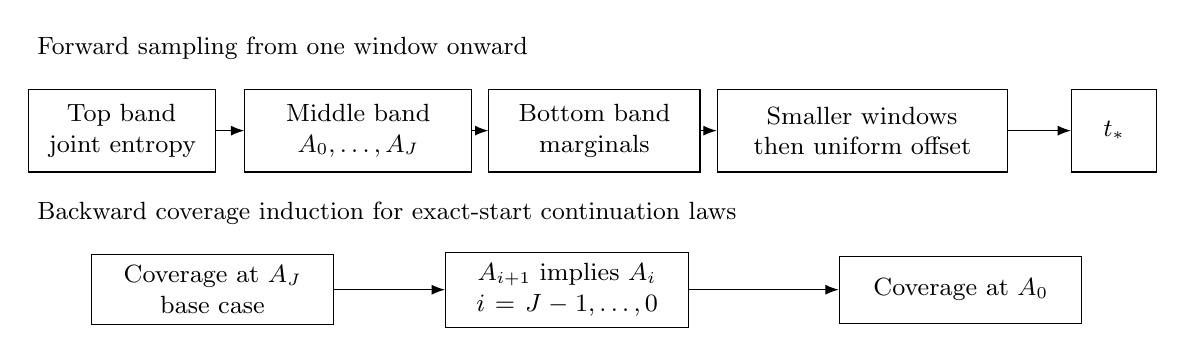
\begin{tikzpicture}[
  >=Latex,font=\small,
  stage/.style={draw,align=center,inner sep=4pt,minimum height=1.05cm},
  proof/.style={draw,align=center,inner sep=4pt,minimum height=0.85cm}]
\node[anchor=west] at (-1.2,1.05)
  {Forward sampling from one window onward};
\node[stage,text width=2.1cm] (top) at (0,0)
  {Top band\\joint entropy};
\node[stage,text width=2.6cm] (mid) at (3.0,0)
  {Middle band\\\(A_0,\ldots,A_J\)};
\node[stage,text width=2.4cm] (bottom) at (6.0,0)
  {Bottom band\\marginals};
\node[stage,text width=3.4cm] (rest) at (9.4,0)
  {Smaller windows\\then uniform offset};
\node[stage,text width=0.8cm] (terminal) at (12.6,0)
  {\(t_*\)};
\draw[->] (top.east) -- (mid.west);
\draw[->] (mid.east) -- (bottom.west);
\draw[->] (bottom.east) -- (rest.west);
\draw[->] (rest.east) -- (terminal.west);

\node[anchor=west] at (-1.2,-1.05)
  {Backward coverage induction for exact-start continuation laws};
\node[proof,text width=2.8cm] (base) at (1.15,-2.02)
  {Coverage at \(A_J\)\\base case};
\node[proof,text width=2.8cm] (step) at (5.65,-2.02)
  {\(A_{i+1}\) implies \(A_i\)\\\(i=J-1,\ldots,0\)};
\node[proof,text width=2.8cm] (goal) at (10.65,-2.02)
  {Coverage at \(A_0\)};
\draw[->] (base.east) -- (step.west);
\draw[->] (step.east) -- (goal.west);
\end{tikzpicture}
\caption{Sampling order and proof order have separate rows. The top row
suppresses individual transitions and shows the common terminal time.
The bottom row proves coverage of the terminal law from every exact
start at each checkpoint. In the step from \(A_{i+1}\) to \(A_i\), fix
the exact start at \(A_i\), run forward to \(A_{i+1}\), then sample
independent continuations conditional on that exact next time.
The induction reverses the checkpoint index; all sampled times move
forward along the fixed walk.}
\label{fig:schedule}
\end{figure}

\subsection{Coverage from every exact checkpoint}\label{sec:checkpoints}
\label{sec:coverage}

We now apply the earlier transfer theorem to the estimates just proved.
The coordinate groups are \(\Z[i]/(\pi)\), their maps are reduction
modulo the two factors over each prime of \(\mathcal B_T\), and the
abstract average \(\overline L\) is exactly \(L_*\).
Averages over signed primes assign equal weight to all \(2k_T\)
prime-factor pairs.

Recall that \((\tau,\beta)\) coverage means that a law on an alphabet
of size \(p\) assigns mass at least \(\tau/p\) outside fewer than
\(p^{1-\beta}\) residues. We use the following floors and exceptional
fractions at the checkpoints already constructed:
\begin{align}
 \tau_0&=\tfrac14,& \delta_i&=2^{-i-6},&
 \tau_{i+1}&=\tau_i+4\delta_i,
 \label{eq:coverage-parameters}\\
 \eta_0&=\tfrac1{100},&&&
 \eta_{i+1}&=\eta_i\delta_i/100.\label{eq:native-eta}
\end{align}
Here \(\beta_i\), \(r_i\), and \(J\) are those of
\eqref{eq:checkpoint-parameters}--\eqref{eq:checkpoint-ranges}.
In particular,
\[
 \tau_i=\frac38-2^{-i-3}<\frac38,\qquad
 \eta_i=100^{-(i+1)}2^{-i(i-1)/2-6i}.
\]
Since \(J=O(M)\), these formulas imply, uniformly over \(0\le i\le J\),
\begin{equation}\label{eq:coverage-parameter-bounds}
 \log(1/\delta_i)=O(M),\qquad
 \eta_i\ge\exp(-O(M^2)),
 \qquad \eta_i\delta_i\beta_{i+1}\ge\exp(-O(M^2)).
\end{equation}
The last estimate is needed only for \(i<J\).

For a specified exact start \(a\) at checkpoint \(A_i\), denote the
terminal residue law of its continuation experiment by
\[
 b_{i,a,\pi}(u)=
 \Pr\{z_{t_*}\bmod\pi=u:
       \text{the remaining schedule is started at }A_i=a\}.
\]
The colon specifies the experiment, including at starts that have
probability zero under the schedule begun at time \(0\).

\begin{proposition}[Terminal residue coverage]\label{prop:coverage}
For all sufficiently large \(M\), uniformly over the batches,
\(0\le i\le J\), and all exact start times \(a\ge0\) at \(A_i\),
all but a fraction at most \(\eta_i\) of the signed primes satisfy
\begin{equation}\label{eq:coverage}
 \#\{u\in\Z[i]/(\pi):b_{i,a,\pi}(u)<\tau_i/p\}
 <p^{1-\beta_i}.
\end{equation}
\end{proposition}

\begin{proof}
We begin at \(A_J\) using the particularly accurate marginal estimate,
then verify every numerical hypothesis of Theorem~\ref{thm:transfer}
for the passage from \(A_{i+1}\) to \(A_i\).

\paragraph{The terminal base.}
Fix any exact start at \(A_J\).
By \eqref{eq:terminal-entropy}, the average relative entropy of the
terminal residue laws from their respective uniform laws is at most
\(e^{-90M^{20}}L_*\).
If a signed prime fails \eqref{eq:coverage}, its low-probability set
has at least \(p^{1-\beta_J}\) elements. The uniform law assigns that
set at least \((1-\tau_J)p^{-\beta_J}\) more mass than its terminal law.
Thus the total variation distance is at least
\[
 (1-\tau_J)p^{-\beta_J}
 \ge c e^{-M^{20}},
\]
using \(p\le2T\), \(\tau_J<3/8\), and
\(\beta_J\log T\le M^{20}\).
Pinsker's inequality in natural logarithms
\cite[Lemma 11.6.1]{CoverThomas} makes each such entropy deficit at least
\(c'e^{-2M^{20}}\).
Averaging the lower bound over the failing signed primes bounds their
fraction by
\[
 C L_*e^{-88M^{20}}
 =\exp(-88M^{20}+O(M))<\eta_J
\]
for all sufficiently large \(M\). This proves the base at every exact
start. The terminal marginal deficit has the accuracy needed to absorb
the power-saving exceptional-set threshold.

\paragraph{The shared data and its cost.}
Suppose coverage has been proved at \(i+1\), and fix an arbitrary
exact start \(A_i=a\). Run the schedule to the next checkpoint and put
\(A=A_{i+1}\) and \(Y=z_A\). Conditional on this exact time \(A\),
repeat the remaining continuation independently
\[
 n_i=\left\lceil T^{6\beta_i/5}\right\rceil
\]
times. Write \(h_1,\ldots,h_{n_i}\) for their physical displacements
from \(Y\), and \(\mathcal H=(h_1,\ldots,h_{n_i})\).
Every \(Y+h_\ell\) has the terminal law from the fixed start \(A_i=a\).
This one data vector is constructed before any auxiliary signed
coordinate subset is selected.

By \eqref{eq:native-data}, every \(h_\ell\) belongs to the same finite
set \(\mathcal D_{i+1}\), even as \(A\) varies. Hence its
\emph{unconditional} entropy in this fixed-start experiment satisfies
\[
 H(\mathcal H)\le n_i\log|\mathcal D_{i+1}|
 \le C_Dn_i T^{r_{i+1}}.
\]
This is not an assertion of independence before conditioning on \(A\).
Combining the support bound with \eqref{eq:checkpoint-entropy} yields
\begin{equation}\label{eq:coverage-data-cost}
 \kappa_i:=\frac{H(\mathcal H)}{s_iL_*}
 \le C_D\exp\left(-\frac45\beta_i\log T+O_D(M^6)\right)
 \le e^{-M^3}.
\end{equation}
Indeed \(n_i\le2T^{6\beta_i/5}\),
\(r_i-r_{i+1}=2\beta_i\), and
\(\beta_i\log T>M^{20}\) for \(i<J\).
The exponent \(4\beta_i/5\) is the margin left after paying for all
\(n_i\) continuations. By Lemma~\ref{lem:conditioning}, the joint
entropy bound and this common cost imply
\begin{equation}\label{eq:coverage-conditional-deficit}
 \E_{p,\pi}\bigl[\log p-H(Y\bmod\pi\mid\mathcal H)\bigr]
 \le \bigl(e^{-cM^3}+\kappa_i\bigr)L_*.
\end{equation}

\paragraph{Checking the transfer inequalities.}
In Theorem~\ref{thm:transfer} take
\[
 (\tau,\delta,\tau',\beta,\beta',\eta,\eta')
 =(\tau_i,\delta_i,\tau_{i+1},\beta_i,\beta_{i+1},
   \eta_i,\eta_{i+1}).
\]
The induction hypothesis supplies the conditional coverage at every
exact value of \(A\). Equation~\eqref{eq:checkpoint-entropy} supplies
its joint entropy input with \(\epsilon_i=e^{-cM^3}\).
The parameter estimates give
\[
 \epsilon_i+\kappa_i
 \le \eta_i\delta_i\beta_{i+1}/16,
 \qquad \eta_{i+1}=\eta_i\delta_i/100,
\]
for sufficiently large \(M\), which are the two entropy budget
requirements. For its concentration requirement, \(p\le2T\) gives
\[
 n_i p^{-\beta_i}
 \ge2^{-\beta_i}T^{\beta_i/5}
 \ge\frac12\exp(M^{20}/5).
\]
It follows that
\(\delta_i^2n_i p^{-\beta_i}/2\ge
\exp(M^{20}/5-O(M))\).
This quantity dominates both
\(\log p\le1.05\,100^M+\log2\) and
\(\log(100/\delta_i)=O(M)\). Consequently
\[
 p\exp(-\delta_i^2n_i p^{-\beta_i}/2)\le\delta_i/100.
\]
The two remaining inequalities are
\[
 \delta_i^{-1}<p^{\beta_{i+1}/2},\qquad
 \log(2e/\delta_i)\le(\beta_{i+1}/4)\log T.
\]
They follow from \(\log(1/\delta_i)=O(M)\) and
\(\beta_{i+1}\log T>M^{20}/2\).
All hypotheses of Theorem~\ref{thm:transfer} now hold. It proves
coverage at \(A_i=a\), and this start was arbitrary. Downward induction
establishes the proposition uniformly over the whole schedule.
\end{proof}

At \(A_0\), the conclusion gives mass at least \(1/(4p)\) outside
fewer than \(p^{199/200}\) residues for at least \(99\%\) of the signed
primes, from every exact start. The next section will use this coverage
and the common terminal-time law to test candidate starting residues
under zero avoidance. There the repeated tests will be independent
conditional on residue vectors, whose laws mix exact starts; that
conditioning will be treated separately.

\section{Zero avoidance costs information}
\label{sec:information}

The sampling and coverage results hold for every self-avoiding walk with
step bound \(D\). We now assume that the walk lies in
\(\mathcal A(\mathcal P_M)\), where \(\mathcal P_M\) is the union of
the prime batches in \eqref{eq:batches}. Thus it avoids zero modulo
both factors of every selected rational prime. This restriction forces
short words of increments to reveal information about the starting
residues. The purpose of this section is to quantify that information
at the common terminal time \(t_*\).

For each batch \(T\), choose independently a uniform subset of
\(q_T\) rational primes, with independent fair signs. Denote all
these auxiliary choices by \(\mathcal C\). They are independent of
the walk-sampling experiment. Entropies below are always computed with
\(\mathcal C\) fixed; an expectation \(\E_{\mathcal C}\) averages
the resulting entropies and does not include the choices as part of
the random data.

For a nonnegative integer time \(t\), write
\[
 W_L(t)=(z_{t+1}-z_t,\ldots,z_{t+L}-z_{t+L-1})
\]
for the next \(L\) increments. Each letter has at most \(K_D\)
possible values. Use the dyadic lengths
\[
 L_T=2^{\lfloor\log_2(T^{2/5})\rfloor},
 \qquad \tfrac12T^{2/5}<L_T\le T^{2/5}.
\]
These lengths are short enough that a word cannot hit one residue twice
modulo a factor of norm \(p\in[T,2T]\), yet long enough that the
displacement from \(A_0(T)\) has negligible entropy compared with the
information in the word. Their dyadic form will let us partition longer
words into shorter ones in Section~\ref{sec:budget}.

Let \(X'_T\) be the selected residue vector of batch \(T\) at
\(z_{t_*}\), and let \(O'_T\) contain the selected residues of all
smaller batches at that same point.

\begin{proposition}[Information cost of one batch]
\label{prop:information-rate}
There is a constant \(c_1>0\), depending only on the fixed schedule
parameters, such that for all sufficiently large \(M\) and every
batch in \eqref{eq:batches},
\begin{equation}
 \frac{1}{L_T}\,
 \E_{\mathcal C}
 I\bigl(X'_T;W_{L_T}(t_*)\mid O'_T\bigr)
 \ge \frac{c_1}{\log T}.
 \label{eq:information-rate}
\end{equation}
The threshold for \(M\) is uniform over all infinite self-avoiding
\(D\)-step walks in \(\mathcal A(\mathcal P_M)\).
\end{proposition}

\begin{proof}
Fix a batch, and abbreviate \(L=L_T\), \(q=q_T\), and
\(A_0=A_0(T)\). Let \(X\) be this batch's selected residue vector
at \(z_{A_0}\), and let \(O\) contain the selected residues of all
smaller batches at \(z_{A_0}\). Their counterparts at \(z_{t_*}\)
are \(X',O'\). Put
\[
 s=z_{t_*}-z_{A_0},\qquad W=W_L(t_*).
\]
We will first show that repeated observations of \((s,W)\) reveal a
fixed fraction of the entropy of \(X\) left after \(O\) is known.
Then we will charge the displacement entropy separately and move the
result to \((X',O',W)\).

By \eqref{eq:global-entropy} and \eqref{eq:smaller-alphabet},
\begin{equation}
 \E_{\mathcal C}H(X\mid O)\ge(1-2e_0)qL_*.
 \label{eq:initial-conditional-entropy}
\end{equation}
Indeed, \(H(X\mid O)\ge H(X)-H(O)\), and the logarithm of the
alphabet size of \(O\) is at most
\(e_0c_0T\le e_0qL_*\). The displacement estimate
\eqref{eq:checkpoint-displacement} gives
\begin{equation}
 H(s)=O_D(T^{r_0})=O_D(T^{1/4}).
 \label{eq:package-shift-entropy}
\end{equation}
Here \(s\) has the original schedule law, which is independent of
\(\mathcal C\).

\paragraph{Testing possible checkpoint residues.}
Choose a sufficiently large fixed constant \(K_0\), specified below,
and set
\[
 m_T=\left\lceil K_0(T/L)\log T\right\rceil.
\]
For fixed \(\mathcal C\), first draw \((O,X)\) with its original
law. Conditional on those values, draw \(m_T\) independent copies
\(P_a=(s_a,W^{(a)})\) of \((s,W)\); write
\(P=(P_1,\ldots,P_{m_T})\). A conditional law at a value of
\((O,X)\) of probability zero may be chosen arbitrarily, since it
does not affect this experiment. Each one-package marginal, together
with \((O,X)\), is the original schedule law.

For a selected factor \(\pi\) of norm \(p\), a candidate
\(x\in\Z[i]/(\pi)\) passes package \(a\) if
\[
 x+s_a+\sum_{h=0}^{l-1}W^{(a)}_h\not\equiv0\pmod\pi
 \qquad(0\le l<L),
\]
where words are indexed from zero and the empty sum is zero.
Let \(\mathcal L_\pi(P)\) be the candidates that pass every
package. The true coordinate \(X_\pi\) always belongs to this
list: the package's exact start has the prescribed residue \(X_\pi\),
and its subsequent positions lie on the zero-avoiding walk. Thus,
almost surely, these lists are nonempty, and
\begin{equation}
 H(X\mid O,P)
 \le \E\sum_{\pi\text{ selected}}\log|\mathcal L_\pi(P)|.
 \label{eq:passing-list-entropy}
\end{equation}
For each realized \((O,P)\), the conditional support of \(X\) is
contained in the Cartesian product of these lists. No independence
between the coordinates of \(X\) is needed.

\paragraph{Coverage after conditioning on residue data.}
The packages just constructed are independent given \((O,X)\),
whereas the continuations used in Proposition~\ref{prop:coverage}
were sampled from an exact checkpoint time. To connect these two
experiments, fix \(\mathcal C\) and a value of \((O,X)\) of
positive probability. Its conditional package law is a mixture over
the posterior exact times \(a\) at \(A_0\). At each such exact
time the future law is the original continuation law: \((O,X)\)
is determined by the time and hence imposes no further condition on
the fresh continuation randomness.
More explicitly, if $K_a$ is the fresh continuation law of $(s,W)$
from the exact time $a$, then for every set $E$ of packages,
\begin{equation}\label{eq:posterior-kernel}
 \Pr\{(s,W)\in E\mid O,X,\mathcal C\}
 =\sum_a\Pr\{A_0=a\mid O,X,\mathcal C\}\,K_a(E).
\end{equation}
The kernel $K_a$ does not depend on the auxiliary prime choices.

Call a selected factor \(\pi\) \emph{favorable} for these residue
data if the posterior probability that \eqref{eq:coverage} holds at
the exact \(A_0\) start is at least \(1/2\). Let \(\chi(a,\pi)\)
indicate failure of coverage for \(\pi\) at the exact start \(a\).
An unfavorable coordinate has posterior bad probability greater than
\(1/2\), so its indicator is at most twice that probability. The
tower property gives
\begin{align}
 \E_{\mathcal C}\E_{O,X}
 \#\{\text{unfavorable selected coordinates}\}
 &\le 2\E_{\mathcal C}\E_{O,X}
       \sum_{\pi\text{ selected}}
       \E[\chi(A_0,\pi)\mid O,X,\mathcal C] \notag\\
 &=2\E_{A_0}\E_{\mathcal C}
       \sum_{\pi\text{ selected}}\chi(A_0,\pi)
 \le 2\eta_0q.
 \label{eq:unfavorable-fraction}
\end{align}
The prior law of \(A_0\) is independent of \(\mathcal C\); its
posterior law need not be. At each exact time,
Proposition~\ref{prop:coverage} bounds the fraction of bad signed
primes by \(\eta_0\), and a uniform signed subset of size \(q\)
therefore contains at most \(\eta_0q\) bad coordinates on average.
This proves the last inequality.

Fix a favorable coordinate and let \(\mu\) be the posterior law
of its exact start. Write \(G\) for the starts where coverage
holds, so \(\mu(G)\ge1/2\). At every \(a\in G\), translating
the terminal residue law by \(z_a\bmod\pi\) gives
\[
 \Pr\{s\equiv-x\pmod\pi\mid A_0=a\}\ge\tau_0/p
\]
for all but fewer than \(p^{1-\beta_0}\) candidates \(x\). Define
\[
 u_x=\mu\left\{a\in G:
     \Pr\{s\equiv-x\pmod\pi\mid A_0=a\}\ge\tau_0/p\right\}.
\]
Averaging the exceptional-set sizes yields
\[
 \sum_{x\in\Z[i]/(\pi)}(\mu(G)-u_x)<p^{1-\beta_0}.
\]
If \(u_x<1/4\), the summand exceeds \(1/4\). Consequently all
but at most \(4p^{1-\beta_0}\) candidates satisfy \(u_x\ge1/4\).
We next show that each of these candidates is unlikely to survive
all the packages.

\paragraph{A short word supplies disjoint chances of rejection.}
For a candidate with \(u_x\ge1/4\), take an exact start counted
by \(u_x\). The smoothing estimate \eqref{eq:smoothing}, applied
at that start, shows for every \(0\le l<L\) that
\[
 \Pr\{z_{t_*+l}-z_{A_0}\equiv-x\pmod\pi\mid A_0=a\}
 \ge\tau_0/(2p).
\]
Indeed \(l\le T_+\), and \(T_+^{-9}\le\tau_0/(2p)\) for all
batches once \(M\) is sufficiently large. Mixing over the posterior
starts gives hit probability at least \(\tau_0/(8p)\) at each
offset.

For a single package, these \(L\) hit events are disjoint. If two
offsets hit, the two walk positions have equal residues modulo
\(\pi\). Their difference is nonzero by self-avoidance, and hence
has length at least \(\sqrt p\). Its length is also at most
\(DL<\sqrt p\), since \(L\le T^{2/5}\) and \(p\ge T\).
This contradiction establishes disjointness. One conditional package
therefore rejects the candidate with probability at least
\(cL/p\), where \(c=\tau_0/8\).

Independence of the packages given \((O,X)\) now yields, for every
favorable coordinate,
\begin{equation}
 \E[|\mathcal L_\pi(P)|\mid O,X]
 \le4p^{1-\beta_0}+p\exp(-cLm_T/p)
 \le5p^{1-\beta_0}.
 \label{eq:passing-list-size}
\end{equation}
Choose the fixed \(K_0\) large enough for the second inequality;
this is possible because \(T\le p\le2T\) and
\(Lm_T/p\ge(K_0/2)\log T\). The choices and the lower threshold
for \(M\) are uniform in the residue data and the walk.

By Jensen's inequality, the expected logarithm of a favorable list's
size is at most \((1-\beta_0)\log p+\log5\). For an unfavorable
coordinate use \(\log p\). Equations
\eqref{eq:passing-list-entropy}--\eqref{eq:passing-list-size} imply
\[
 \begin{aligned}
 \E_{\mathcal C}H(X\mid O,P)
 &\le(1-\beta_0)qL_*
       +2\eta_0\beta_0q\log(2T)+q\log5\\
 &\le(1-\beta_0/2)qL_*
 \end{aligned}
\]
for large \(M\). Here \(\eta_0=1/100\),
\(L_*\ge\log T\), and \(\log5/L_*\to0\).
Subtracting this bound from \eqref{eq:initial-conditional-entropy}
and using \(e_0=\beta_0/50\), we obtain
\begin{equation}
 \E_{\mathcal C}I(X;P\mid O)\ge(\beta_0/3)qL_*.
 \label{eq:package-information-lower}
\end{equation}
Repeated tests have thus exposed a fixed fraction of the checkpoint
residue entropy. It remains to place the cost in the terminal word
itself, since only terminal words will enter the common budget.

\paragraph{Transporting the information to the terminal time.}
For fixed \(\mathcal C\), conditional independence gives
\[
 \begin{aligned}
 I(X;P\mid O)
 &=H(P\mid O)-\sum_{a=1}^{m_T}H(P_a\mid O,X)\\
 &\le\sum_{a=1}^{m_T}I(X;P_a\mid O)
 =m_TI(X;s,W\mid O).
 \end{aligned}
\]
There are two costs in removing the displacement. First,
\(I(X;s\mid O)\le H(s)\). Second, given the full Gaussian-integer
displacement \(s\), residue addition is a bijection between
\((O,X)\) and \((O',X')\), so
\[
 I(X;W\mid O,s)=I(X';W\mid O',s).
\]
For any finite variables,
\[
 I(A;B\mid C,S)-I(A;B\mid C)
 =I(A;S\mid B,C)-I(A;S\mid C)\le H(S).
\]
Removing the conditioning on \(s\) therefore costs at most another
\(H(s)\). In total,
\begin{equation}
 I(X;s,W\mid O)\le I(X';W\mid O')+2H(s).
 \label{eq:translate-information}
\end{equation}
The one-package marginal is the original schedule law. Thus the
variables on the right are precisely
\(X'_T,O'_T,W_{L_T}(t_*)\), under the same terminal law as for
every other batch.

Finally, \(qL_*\ge c_0T\) and
\(m_T\le2K_0(T/L)\log T\) for large \(T\). Equations
\eqref{eq:package-information-lower},
\eqref{eq:translate-information}, and
\eqref{eq:package-shift-entropy} give
\[
 \E_{\mathcal C}I(X';W\mid O')
 \ge\frac{\beta_0c_0}{6K_0}\frac{L}{\log T}-O_D(T^{1/4}).
\]
Since \(T^{1/4}=o(L/\log T)\), this proves
\eqref{eq:information-rate} with, for example,
\(c_1=\beta_0c_0/(12K_0)\).
\end{proof}

\section{The common-law entropy budget}
\label{sec:budget}

Each batch now charges a positive amount of information to an increment
word. We must show that these charges can be added, despite the different
word lengths. The residue vectors will be nested in increasing batch
order. Knowing the earlier increments updates the residue vector to the
start of each new block, while the smoothing of \(t_*\) compares that
block's law with the law at \(t_*\). These two facts make the entropy
differences telescope.

\begin{lemma}[A common-law entropy telescope]
\label{lem:telescope}
For every fixed collection \(\mathcal C\) of prime choices,
\begin{equation}
 \sum_T\frac{I(X'_T;W_{L_T}(t_*)\mid O'_T)}{L_T}
 \le\log K_D+o(1),
 \label{eq:information-telescope}
\end{equation}
where the error tends to zero uniformly over the choices and the walks
as \(M\to\infty\).
\end{lemma}

\begin{proof}
Order the batches as \(T_1<\cdots<T_{n_B}\), and put
\(L_j=L_{T_j}\). For every time \(t\), let \(Q_j(t)\) contain
all selected residues from batches through \(T_j\) at \(z_t\);
let \(Q_0\) be empty. Define
\[
 a_j=\frac{H(W_{L_j}(t_*)\mid Q_{j-1}(t_*))}{L_j},
 \qquad
 b_j=\frac{H(W_{L_j}(t_*)\mid Q_j(t_*))}{L_j}.
\]
The \(j\)-th charge is \(a_j-b_j\). We claim that the initial
entropy rate for batch \(j+1\) is bounded, up to a small error,
by the remaining rate \(b_j\) after batch \(j\).

Both lengths are powers of two and \(L_j\le L_{j+1}\), so
\(L_j\) divides \(L_{j+1}\). Partition the longer word into
blocks of length \(L_j\). For a block starting at offset \(a\),
\(Q_j(t_*)\) and the preceding increments determine
\(Q_j(t_*+a)\), by adding their sum in every residue coordinate.
The entropy chain rule, followed by removal of conditioning, gives
\[
 H(W_{L_{j+1}}(t_*)\mid Q_j(t_*))
 \le\sum_{\substack{0\le a<L_{j+1}\\L_j\mid a}}
 H(W_{L_j}(t_*+a)\mid Q_j(t_*+a)).
\]

Both the block and its starting residue vector are deterministic
functions of the starting time on the fixed walk. By
\eqref{eq:smoothing}, their joint law at \(t_*+a\) differs from
that at \(t_*\) in total variation by at most \(T_+^{-9}\), since
\(a<L_{j+1}\le T_+^{2/5}\le T_+\). This is approximate invariance
of the sampled time law; no stationarity of the walk is assumed.

The logarithm of the full residue alphabet is at most
\[
 \sum_T k_T\log(2T)=O(T_+),
\]
by \eqref{eq:prime-count} and geometric spacing of the batches.
The block alphabet contributes at most
\(L_j\log K_D=O_D(T_+)\). Lemma~\ref{lem:continuity} therefore
gives, uniformly in the block and in \(\mathcal C\),
\[
 \begin{aligned}
 H(W_{L_j}(t_*+a)\mid Q_j(t_*+a))
 &\le H(W_{L_j}(t_*)\mid Q_j(t_*))+\epsilon_M,\\
 \epsilon_M&=O_D(T_+^{-7}).
 \end{aligned}
\]
Indeed the continuity bound is
\(2h(T_+^{-9})+O_D(T_+^{-8})\), which is smaller than the displayed
error for sufficiently large \(M\). Dividing the block sum by
\(L_{j+1}\) now yields
\[
 a_{j+1}\le b_j+\epsilon_M/L_j\le b_j+\epsilon_M.
\]
There are \(n_B=O(\log T_+)\) batches, so
\[
 \sum_{j=1}^{n_B}(a_j-b_j)
 \le a_1-b_{n_B}+(n_B-1)\epsilon_M
 \le\log K_D+o(1).
\]
Here \(b_{n_B}\ge0\), and the \(K_D\)-letter increment alphabet
gives \(a_1\le\log K_D\).
\end{proof}

This telescope is methodologically related to Tao's entropy-decrement
argument~\cite[Section~3, Equation~(40) and Lemma~17]{TaoEntropyDecrement}:
approximate translation invariance and conditional block subadditivity
limit accumulated information. Here the information charges arise from
zero avoidance across nested prime batches, and the preceding proof
establishes the required bound for our single terminal-time law.

\begin{proof}[Proof of Theorem~\ref{thm:sieve}]
Fix \(D\) and all schedule constants. Suppose that, for a given
sufficiently large \(M\), an infinite self-avoiding \(D\)-step walk
lies in \(\mathcal A(\mathcal P_M)\). Averaging
Lemma~\ref{lem:telescope} over \(\mathcal C\) and applying
Proposition~\ref{prop:information-rate} gives
\begin{equation}
 c_1\sum_T\frac1{\log T}\le\log K_D+o(1).
 \label{eq:final-information-bound}
\end{equation}

For each \(\lceil M/2\rceil\le m\le M\), the interval
\([X_m,1.05X_m]\) contains at least \(cX_m/\log B\) of the
numbers \(\log T=j\log B\), for an absolute \(c>0\) and all
sufficiently large \(M\). Its contribution to the sum in
\eqref{eq:final-information-bound} is at least
\(c/(1.05\log B)\). There are order \(M\) such disjoint
intervals. Their total contribution tends to infinity, whereas
\(c_1\), \(B\), and \(K_D\) are fixed. This contradicts
\eqref{eq:final-information-bound} once \(M\) is sufficiently large.

Every estimate and every lower threshold for \(M\) is uniform over
the hypothetical avoiding walks. Choose one such \(M\), depending
only on \(D\), and set \(\mathcal P_D=\mathcal P_M\). This is
one finite set of rational primes, with both factors imposed in
\(\mathcal A(\mathcal P_D)\), for which no infinite avoiding walk
exists. The auxiliary signed subsets were used only to average the
information inequalities; they do not make the final sieve depend on
the walk. This proves Theorem~\ref{thm:sieve} and supplies the input
to the periodicity argument in Section~\ref{sec:consequences}.
\end{proof}

\begin{thebibliography}{99}

\bibitem{BLM}
S. Boucheron, G. Lugosi, and P. Massart,
\emph{Concentration Inequalities: A Nonasymptotic Theory of Independence},
Oxford University Press, Oxford, 2013.
\url{https://doi.org/10.1093/acprof:oso/9780199535255.001.0001}.

\bibitem{Conrad}
K. Conrad, \emph{The Gaussian Integers}, expository notes.
\url{https://kconrad.math.uconn.edu/blurbs/ugradnumthy/Zinotes.pdf}
(accessed 27 September 2026).

\bibitem{CoverThomas}
T. M. Cover and J. A. Thomas,
\emph{Elements of Information Theory}, second edition,
Wiley-Interscience, Hoboken, NJ, 2006.
\url{https://doi.org/10.1002/047174882X}.

\bibitem{Erdos1977}
P. Erd\H{o}s,
Problems and results on combinatorial number theory III,
in \emph{Number Theory Day} (Rockefeller University, New York, 1976),
Lecture Notes in Mathematics, vol.~626,
Springer, Berlin, 1977, pp.~43--72.
\url{https://www.renyi.hu/~p_erdos/1977-27.pdf}.

\bibitem{GethnerStark}
E. Gethner and H. M. Stark,
Periodic Gaussian moats,
\emph{Experimental Mathematics} \textbf{6} (1997), no.~4, 289--292.
\url{https://doi.org/10.1080/10586458.1997.10504616}.

\bibitem{GethnerWagonWick}
E. Gethner, S. Wagon, and B. Wick,
A stroll through the Gaussian primes,
\emph{American Mathematical Monthly} \textbf{105} (1998), no.~4, 327--337.
\url{https://doi.org/10.1080/00029890.1998.12004889}.

\bibitem{Harper}
L. H. Harper,
Optimal assignments of numbers to vertices,
\emph{Journal of the Society for Industrial and Applied Mathematics}
\textbf{12} (1964), no.~1, 131--135.
\url{https://doi.org/10.1137/0112012}.

\bibitem{Hatcher}
A. Hatcher, \emph{Algebraic Topology},
Cambridge University Press, Cambridge, 2002.
\url{https://pi.math.cornell.edu/~hatcher/AT/ATpage.html}.

\bibitem{Hoeffding}
W. Hoeffding,
Probability inequalities for sums of bounded random variables,
\emph{Journal of the American Statistical Association}
\textbf{58} (1963), no.~301, 13--30.
\url{https://doi.org/10.1080/01621459.1963.10500830}.

\bibitem{Lugosi}
G. Lugosi, \emph{Concentration-of-measure inequalities},
lecture notes, June 25, 2009.
\href{https://www.upf.edu/documents/298368705/0/anu.pdf/7c62a169-bd53-4c93-b192-d1a75373ce40?t=1745790909783}{Author-hosted lecture notes}.

\bibitem{Selberg}
A. Selberg,
An elementary proof of the prime-number theorem for arithmetic progressions,
\emph{Canadian Journal of Mathematics} \textbf{2} (1950), 66--78.
\url{https://doi.org/10.4153/CJM-1950-007-5}.

\bibitem{TaoEntropyDecrement}
T. Tao,
The logarithmically averaged Chowla and Elliott conjectures for two-point correlations,
\emph{Forum of Mathematics, Pi} \textbf{4} (2016), e8, 36 pp.
\url{https://doi.org/10.1017/fmp.2016.6}.

\bibitem{Tsuchimura}
N. Tsuchimura,
Computational results for Gaussian moat problem,
\emph{IEICE Transactions on Fundamentals of Electronics, Communications
and Computer Sciences} \textbf{E88-A} (2005), no.~5, 1267--1273.
\url{https://doi.org/10.1093/ietfec/e88-a.5.1267}.

\bibitem{Vardi}
I. Vardi,
Prime percolation,
\emph{Experimental Mathematics} \textbf{7} (1998), no.~3, 275--289.
\url{https://doi.org/10.1080/10586458.1998.10504373}.

\end{thebibliography}

\end{document}
